\documentclass[11pt]{article}

\usepackage[a4paper,margin=1in]{geometry}
\usepackage[T1]{fontenc}
\usepackage[utf8]{inputenc}
\usepackage{amsmath}
\usepackage{graphicx}
\usepackage{float}
\usepackage{booktabs}
\usepackage{tabularx}
\usepackage{array}
\usepackage{subcaption}
\usepackage{hyperref}
\usepackage{enumitem}

\hypersetup{
    colorlinks=true,
    linkcolor=blue,
    citecolor=blue,
    urlcolor=blue
}

\graphicspath{{figures/latency/}}

\title{Finite-Blocklength Latency Minimization for Uplink and Downlink Communications:\\Method Results: Latency}
\author{}
\date{July 6, 2026}

\begin{document}

\maketitle

\begin{abstract}
This document presents the latency results for uplink and downlink using the
same terminology as the companion theory report. Throughout the discussion, the
\emph{Training Only Method} is used as the benchmark for the
\emph{Training + Testing Method}. The main outcome is different across the two
links. In the downlink, the benchmark remains clearly stronger, especially in
payload completion, where final total latency is \(0.0358\) s for the
\emph{Training Only Method} and \(0.0735\) s for the \emph{Training + Testing
Method}. In the uplink, the gap is much smaller, and under continuous
communication both methods finish with the same total latency, \(0.027333\) s.
\end{abstract}

\section{Scope and Naming}

This document is latency-only. The terminology is aligned with
the companion theory report:
\begin{itemize}[leftmargin=1.5em]
    \item \textbf{Training Only Method}: direct online optimization during scheduling,
    \item \textbf{Training + Testing Method}: a separate training stage followed by testing-stage inference,
    \item \textbf{Payload completion}: the scenario where each user continues until its remaining payload is exhausted, and
    \item \textbf{Continuous communication}: the scenario with a prescribed communication horizon and prescribed blockwise bits sequence.
\end{itemize}

The \emph{Training Only Method} is treated as the benchmark, and the
\emph{Training + Testing Method} is evaluated against it.

\section{Downlink}

The downlink results show the clearest gap between the benchmark and the
\emph{Training + Testing Method}. Table~\ref{tab:downlink-latency-summary}
summarizes the scenario-level totals.

\begin{table}[ht]
\centering
\scriptsize
\setlength{\tabcolsep}{4pt}
\caption{Downlink latency summary}
\label{tab:downlink-latency-summary}
\renewcommand{\arraystretch}{1.15}
\begin{tabularx}{\textwidth}{>{\raggedright\arraybackslash}p{0.21\textwidth} >{\raggedright\arraybackslash}p{0.24\textwidth} >{\centering\arraybackslash}p{0.14\textwidth} >{\centering\arraybackslash}p{0.14\textwidth} >{\centering\arraybackslash}p{0.13\textwidth} X}
\toprule
Scenario & Method & Init. total (s) & Final total (s) & Final avg (s) & Red. (\%) \\
\midrule
Payload completion & Training Only & 0.3050 & 0.0358 & 0.01193 & 88.26 \\
Payload completion & Training + Testing & 0.3050 & 0.0735 & 0.02451 & 75.89 \\
Continuous communication & Training Only & 0.0633 & 0.0436 & 0.01453 & 31.16 \\
Continuous communication & Training + Testing & 0.0633 & 0.0573 & 0.01909 & 9.58 \\
\bottomrule
\end{tabularx}
\end{table}

\subsection{Payload Completion Results and Comparison}

Downlink payload completion is the strongest benchmark test. The
\emph{Training Only Method} reduces total latency from \(0.3050\) s to
\(0.0358\) s, while the \emph{Training + Testing Method} reaches \(0.073533\)
s. The testing-stage method therefore improves substantially, but it does not
yet match the benchmark.

The per-user pattern in Figure~\ref{fig:dl-payload-latency} clarifies where
that gap comes from. User 1 is already close to the benchmark, with
\(0.009333\) s versus \(0.010933\) s. The main shortfall is on users 0 and 2.
For user 0, the final latency increases from \(0.013200\) s at the benchmark
to \(0.028467\) s for the \emph{Training + Testing Method}. For user 2, it
increases from \(0.013267\) s to \(0.034133\) s. The main limitation is
therefore the slower-user tail.

\begin{figure}[ht]
\centering
\begin{subfigure}[t]{0.48\textwidth}
    \centering
    
\includegraphics[width=\textwidth]{dl_payload_training_only.png}
    \caption{Training Only Method}
\end{subfigure}
\hfill
\begin{subfigure}[t]{0.48\textwidth}
    \centering
    
\includegraphics[width=\textwidth]{dl_payload_training_testing.png}
    \caption{Training + Testing Method}
\end{subfigure}
\caption{Downlink payload-completion latency comparison. The \emph{Training Only Method} compresses all three user latencies strongly, while the \emph{Training + Testing Method} leaves a visibly longer tail on users 0 and 2.}
\label{fig:dl-payload-latency}
\end{figure}

\subsection{Continuous Communication Results and Comparison}

The benchmark also remains better in downlink continuous communication. Total
latency falls from \(0.063333\) s to \(0.043600\) s under the
\emph{Training Only Method}, whereas the \emph{Training + Testing Method}
reaches \(0.057267\) s.

Figure~\ref{fig:dl-continuous-latency} shows that the gap is again structural
rather than cosmetic. User 0 stays at \(0.016667\) s in both cases. User 1 is
reduced in both methods, but the benchmark reaches \(0.009333\) s while the
\emph{Training + Testing Method} reaches \(0.013933\) s. The largest gap is on
user 2: the benchmark shortens it to \(0.017600\) s, while the
\emph{Training + Testing Method} leaves it at \(0.026667\) s. The benchmark
advantage therefore comes from stronger compression of the longer latencies.

\begin{figure}[ht]
\centering
\begin{subfigure}[t]{0.48\textwidth}
    \centering
    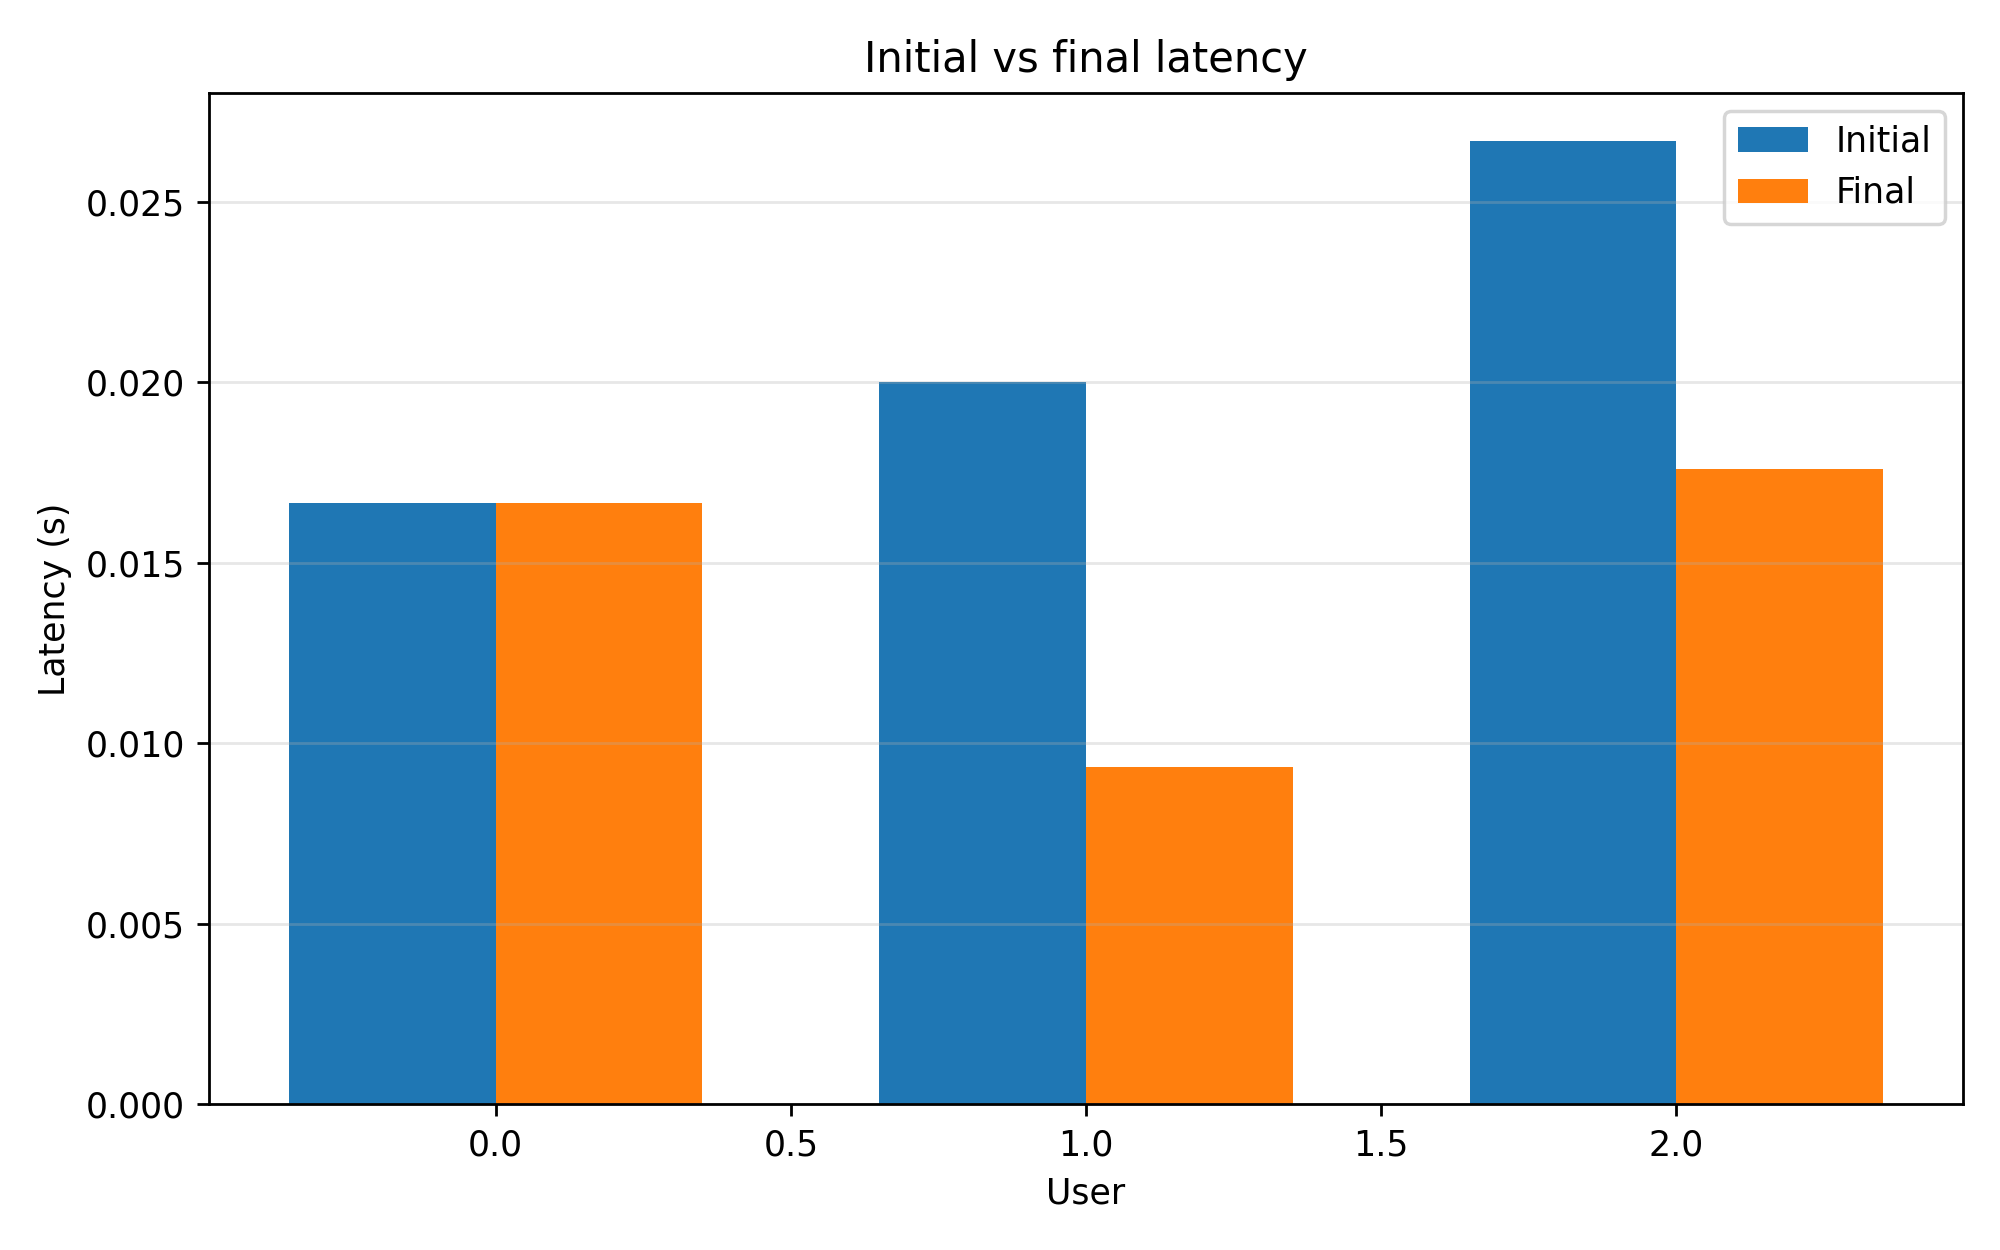
\includegraphics[width=\textwidth]{dl_continuous_training_only.png}
    \caption{Training Only Method}
\end{subfigure}
\hfill
\begin{subfigure}[t]{0.48\textwidth}
    \centering
    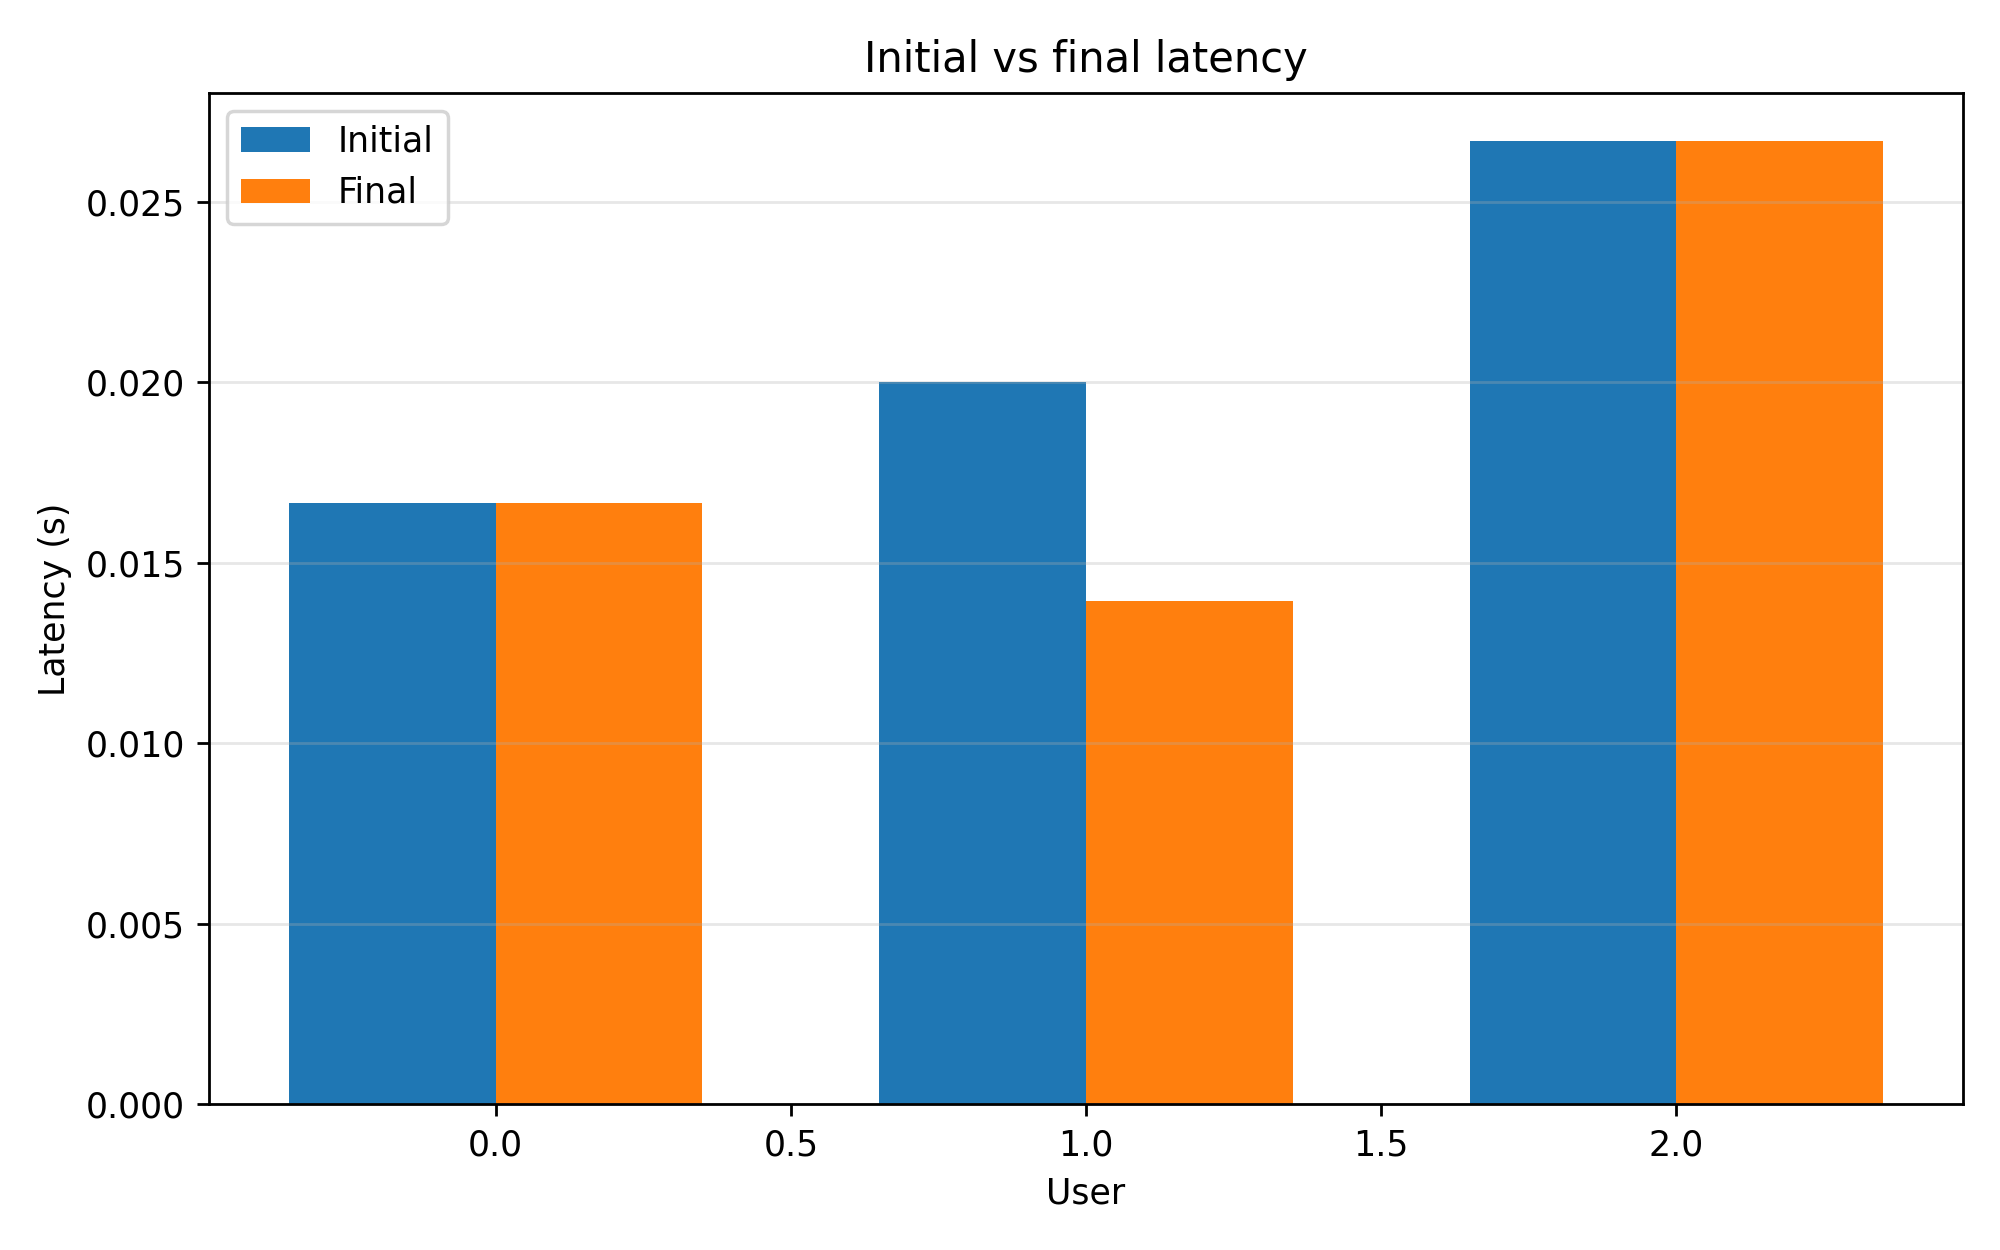
\includegraphics[width=\textwidth]{dl_continuous_training_testing.png}
    \caption{Training + Testing Method}
\end{subfigure}
\caption{Downlink continuous-communication latency comparison. The \emph{Training Only Method} achieves visible compression on users 1 and 2, whereas the \emph{Training + Testing Method} mainly improves user 1 and leaves the overall latency profile much closer to the initial one.}
\label{fig:dl-continuous-latency}
\end{figure}

\section{Uplink}

In the uplink, the \emph{Training + Testing Method} stays much closer to the
benchmark. Table~\ref{tab:uplink-latency-summary} shows that the latency gap is
small in both scenarios.

\begin{table}[ht]
\centering
\scriptsize
\setlength{\tabcolsep}{4pt}
\caption{Uplink latency summary}
\label{tab:uplink-latency-summary}
\renewcommand{\arraystretch}{1.15}
\begin{tabularx}{\textwidth}{>{\raggedright\arraybackslash}p{0.21\textwidth} >{\raggedright\arraybackslash}p{0.24\textwidth} >{\centering\arraybackslash}p{0.14\textwidth} >{\centering\arraybackslash}p{0.14\textwidth} >{\centering\arraybackslash}p{0.13\textwidth} X}
\toprule
Scenario & Method & Init. total (s) & Final total (s) & Final avg (s) & Red. (\%) \\
\midrule
Payload completion & Training Only & 0.0307 & 0.0247 & 0.00822 & 19.74 \\
Payload completion & Training + Testing & 0.0307 & 0.0252 & 0.00840 & 18.00 \\
Continuous communication & Training Only & 0.0331 & 0.0273 & 0.00911 & 17.50 \\
Continuous communication & Training + Testing & 0.0331 & 0.0273 & 0.00911 & 17.50 \\
\bottomrule
\end{tabularx}
\end{table}

\subsection{Payload Completion Results and Comparison}

In uplink payload completion, the benchmark and the
\emph{Training + Testing Method} are nearly tied. Final total latency is
\(0.024667\) s for the benchmark and \(0.025200\) s for the
\emph{Training + Testing Method}.

Figure~\ref{fig:ul-payload-latency} confirms this close match. User 0 finishes
very slightly better under the \emph{Training + Testing Method}
\((0.004467\ \text{s})\) than under the \emph{Training Only Method}
\((0.004533\ \text{s})\). User 2 also ends almost identically
\((0.012133\ \text{s} \text{ versus } 0.012200\ \text{s})\). The main visible
difference is user 1, where the \emph{Training Only Method} reaches
\(0.007933\) s instead of \(0.008600\) s. This user-1 gap is what gives the
benchmark the better total latency, but the margin remains small.

\begin{figure}[ht]
\centering
\begin{subfigure}[t]{0.48\textwidth}
    \centering
    
\includegraphics[width=\textwidth]{ul_payload_training_only.png}
    \caption{Training Only Method}
\end{subfigure}
\hfill
\begin{subfigure}[t]{0.48\textwidth}
    \centering
    
\includegraphics[width=\textwidth]{ul_payload_training_testing.png}
    \caption{Training + Testing Method}
\end{subfigure}
\caption{Uplink payload-completion latency comparison. Both methods shorten all three users and end with nearly the same per-user latency profile.}
\label{fig:ul-payload-latency}
\end{figure}

\subsection{Continuous Communication Results and Comparison}

The uplink continuous-communication scenario is the closest benchmark match in
the document. Both methods finish with the same total latency, \(0.027333\) s,
and the same final average latency, \(0.009111\) s.

The per-user bars in Figure~\ref{fig:ul-continuous-latency} show that the tie
still hides small redistributions. The \emph{Training + Testing Method} is
slightly better on user 0, reaching \(0.005133\) s instead of \(0.005267\) s,
and on user 2, reaching \(0.013067\) s instead of \(0.013400\) s. The
\emph{Training Only Method} is better on user 1, reaching \(0.008667\) s
instead of \(0.009133\) s. Those differences cancel almost exactly in the
total, so at system level the \emph{Training + Testing Method} matches the
benchmark in this case.

\begin{figure}[ht]
\centering
\begin{subfigure}[t]{0.48\textwidth}
    \centering
    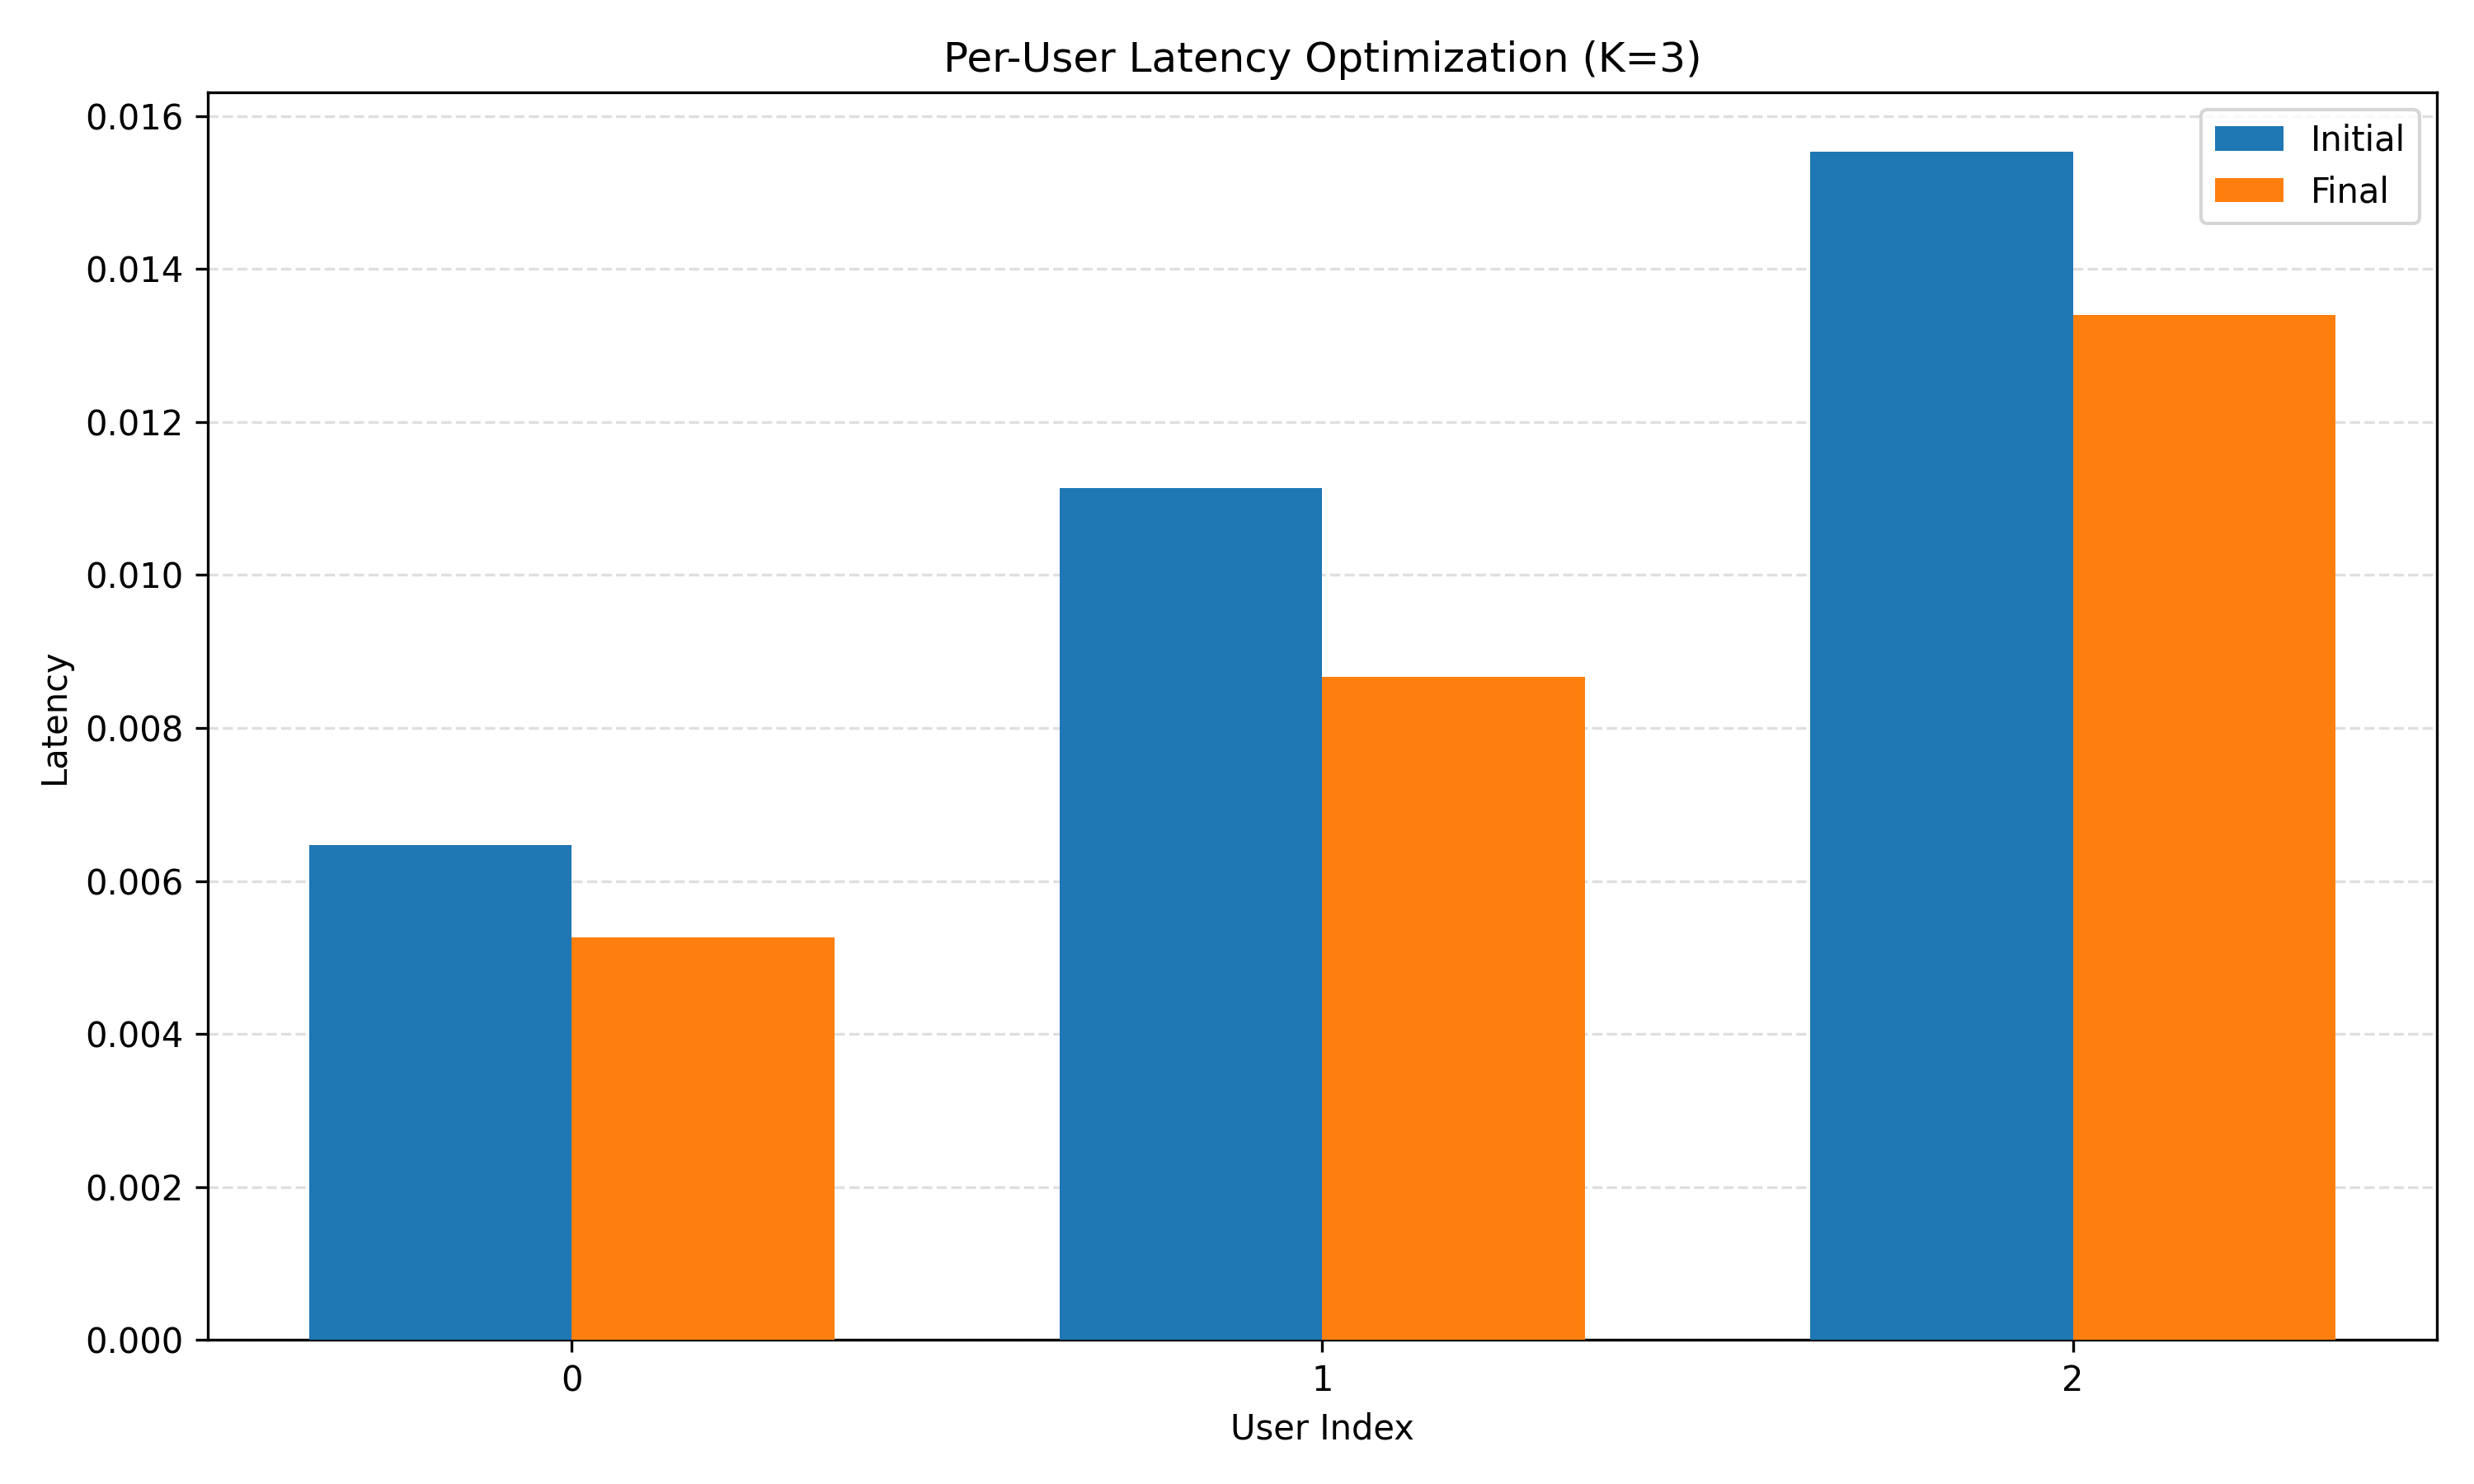
\includegraphics[width=\textwidth]{ul_continuous_training_only.png}
    \caption{Training Only Method}
\end{subfigure}
\hfill
\begin{subfigure}[t]{0.48\textwidth}
    \centering
    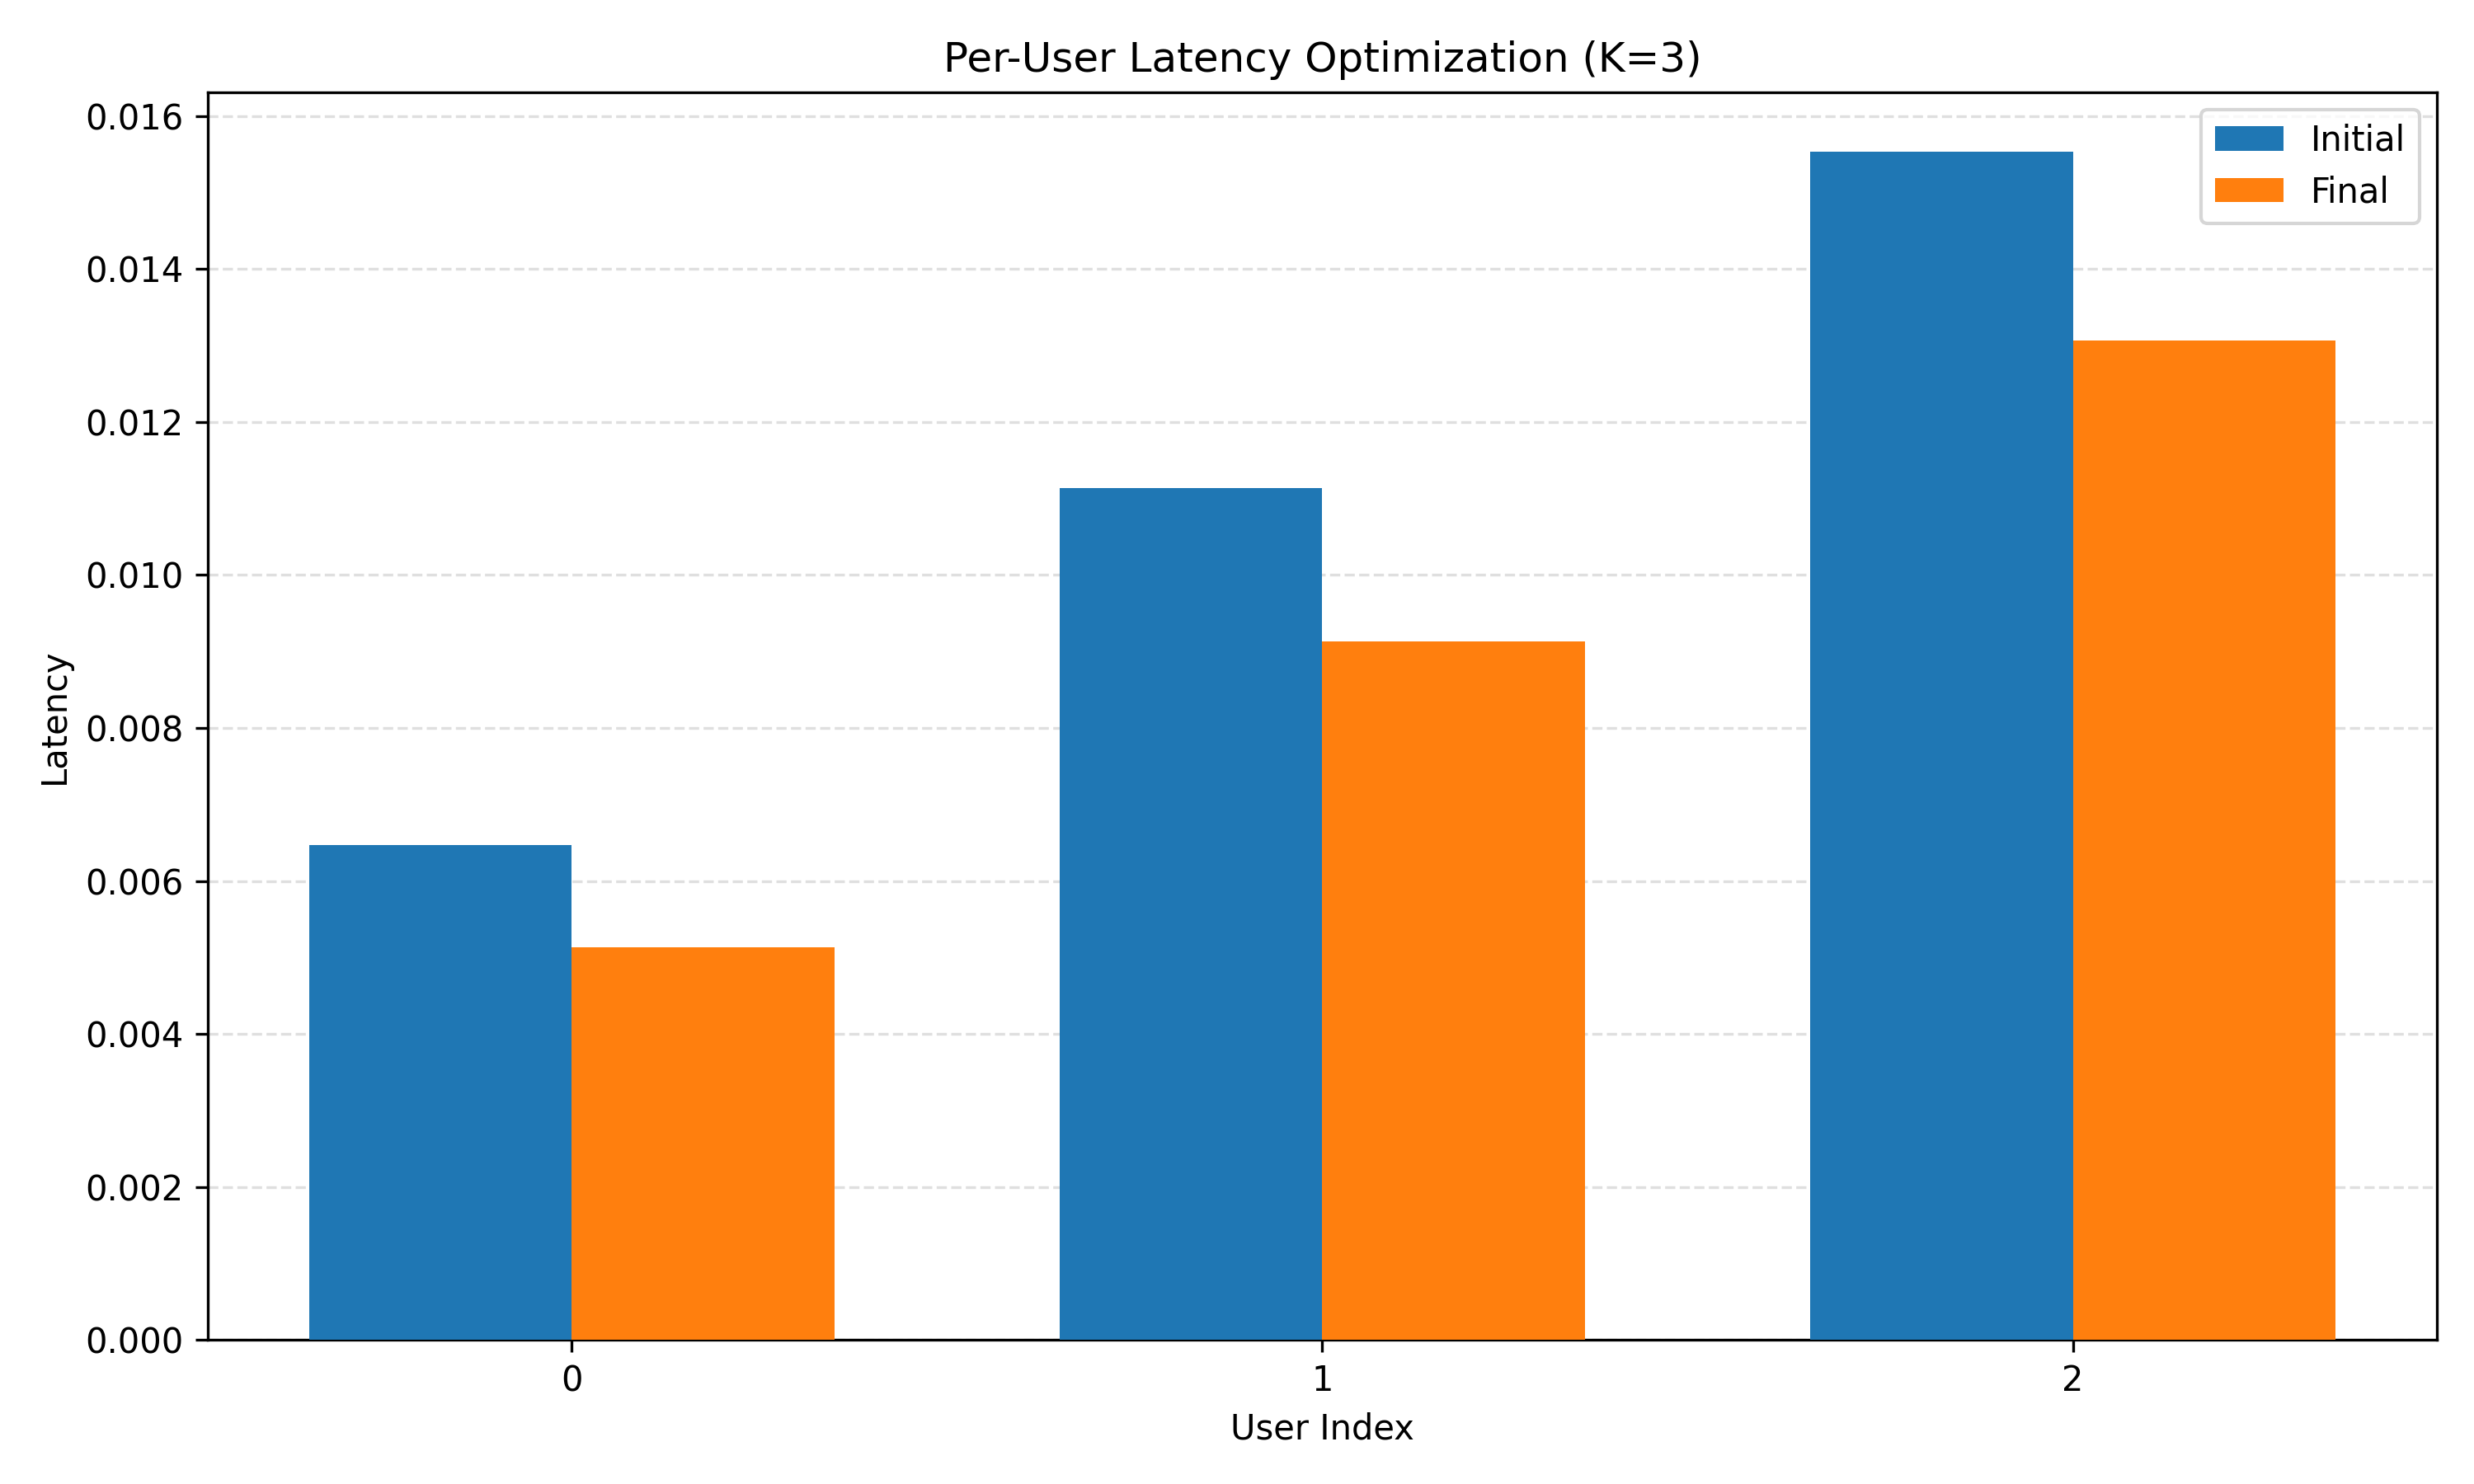
\includegraphics[width=\textwidth]{ul_continuous_training_testing.png}
    \caption{Training + Testing Method}
\end{subfigure}
\caption{Uplink continuous-communication latency comparison. The total latency is identical across the two methods, with only small user-level reallocations inside that tie.}
\label{fig:ul-continuous-latency}
\end{figure}

\section{Asynchronality Results}

The asynchronality results are summarized across both links and both scenarios
in Tables~\ref{tab:downlink-async-summary} and
\ref{tab:uplink-async-summary}. The benchmark remains the clearest reference.
Its strongest synchronization gain appears in downlink payload completion,
while the uplink results are much closer across the two methods.

\begin{table}[H]
\centering
\scriptsize
\setlength{\tabcolsep}{4pt}
\caption{Downlink asynchronality summary}
\label{tab:downlink-async-summary}
\renewcommand{\arraystretch}{1.15}
\begin{tabularx}{\textwidth}{>{\raggedright\arraybackslash}p{0.21\textwidth} >{\raggedright\arraybackslash}p{0.24\textwidth} >{\centering\arraybackslash}p{0.14\textwidth} >{\centering\arraybackslash}p{0.14\textwidth} X}
\toprule
Scenario & Method & Init. async. (s) & Final async. (s) & Red. (\%) \\
\midrule
Payload completion & Training Only & 0.131600 & 0.007867 & 94.02 \\
Payload completion & Training + Testing & 0.131600 & 0.046400 & 64.74 \\
Continuous communication & Training Only & 0.020000 & 0.016533 & 17.33 \\
Continuous communication & Training + Testing & 0.020000 & 0.025467 & -27.33 \\
\bottomrule
\end{tabularx}
\end{table}

\begin{table}[H]
\centering
\scriptsize
\setlength{\tabcolsep}{4pt}
\caption{Uplink asynchronality summary}
\label{tab:uplink-async-summary}
\renewcommand{\arraystretch}{1.15}
\begin{tabularx}{\textwidth}{>{\raggedright\arraybackslash}p{0.21\textwidth} >{\raggedright\arraybackslash}p{0.24\textwidth} >{\centering\arraybackslash}p{0.14\textwidth} >{\centering\arraybackslash}p{0.14\textwidth} X}
\toprule
Scenario & Method & Init. async. (s) & Final async. (s) & Red. (\%) \\
\midrule
Payload completion & Training Only & 0.016667 & 0.015333 & 8.00 \\
Payload completion & Training + Testing & 0.016667 & 0.015333 & 8.00 \\
Continuous communication & Training Only & 0.018133 & 0.016267 & 10.29 \\
Continuous communication & Training + Testing & 0.018133 & 0.015867 & 12.50 \\
\bottomrule
\end{tabularx}
\end{table}

\subsection{Downlink}

Downlink payload completion is the clearest synchronization win for the
\emph{Training Only Method}. Its asynchronality sum falls to \(0.007867\) s,
compared with \(0.046400\) s for the \emph{Training + Testing Method}. The
gap remains visible in the figure pair, where the benchmark finishes with a
much tighter final spread.

\begin{figure}[H]
\centering
\begin{subfigure}[t]{0.48\textwidth}
    \centering
    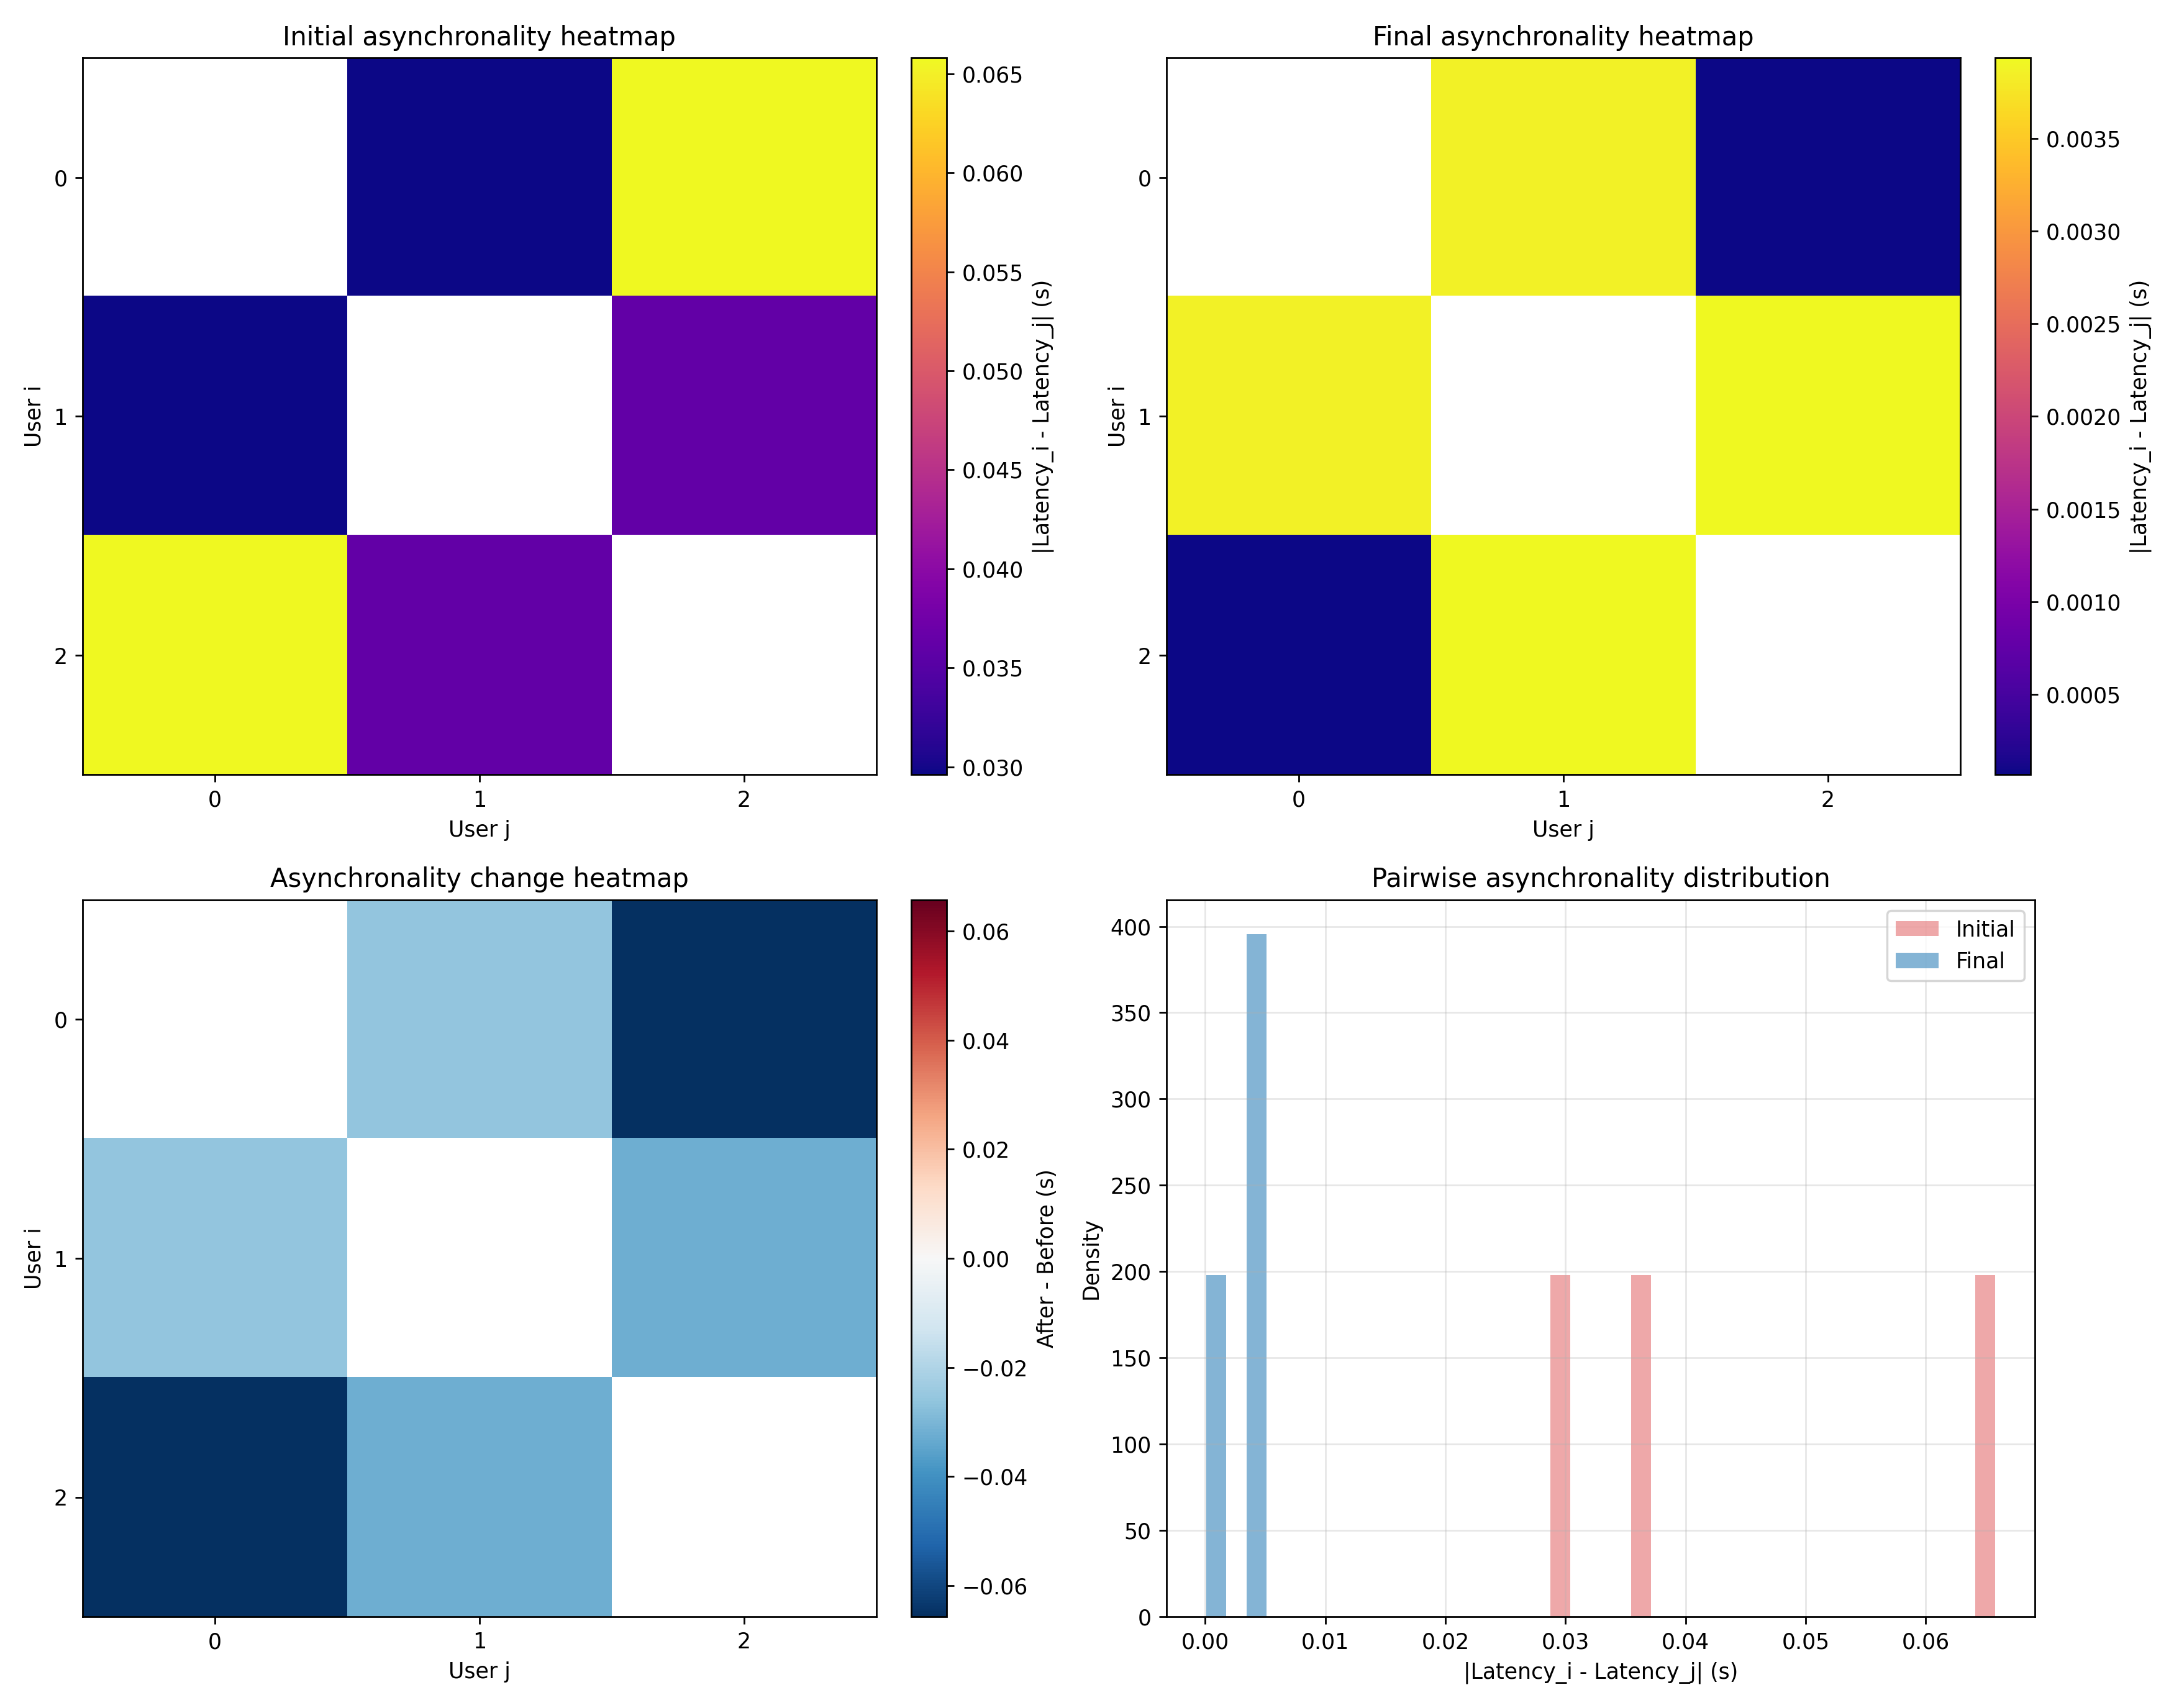
\includegraphics[width=\textwidth]{dl_payload_async_training_only.png}
    \caption{Training Only Method}
\end{subfigure}
\hfill
\begin{subfigure}[t]{0.48\textwidth}
    \centering
    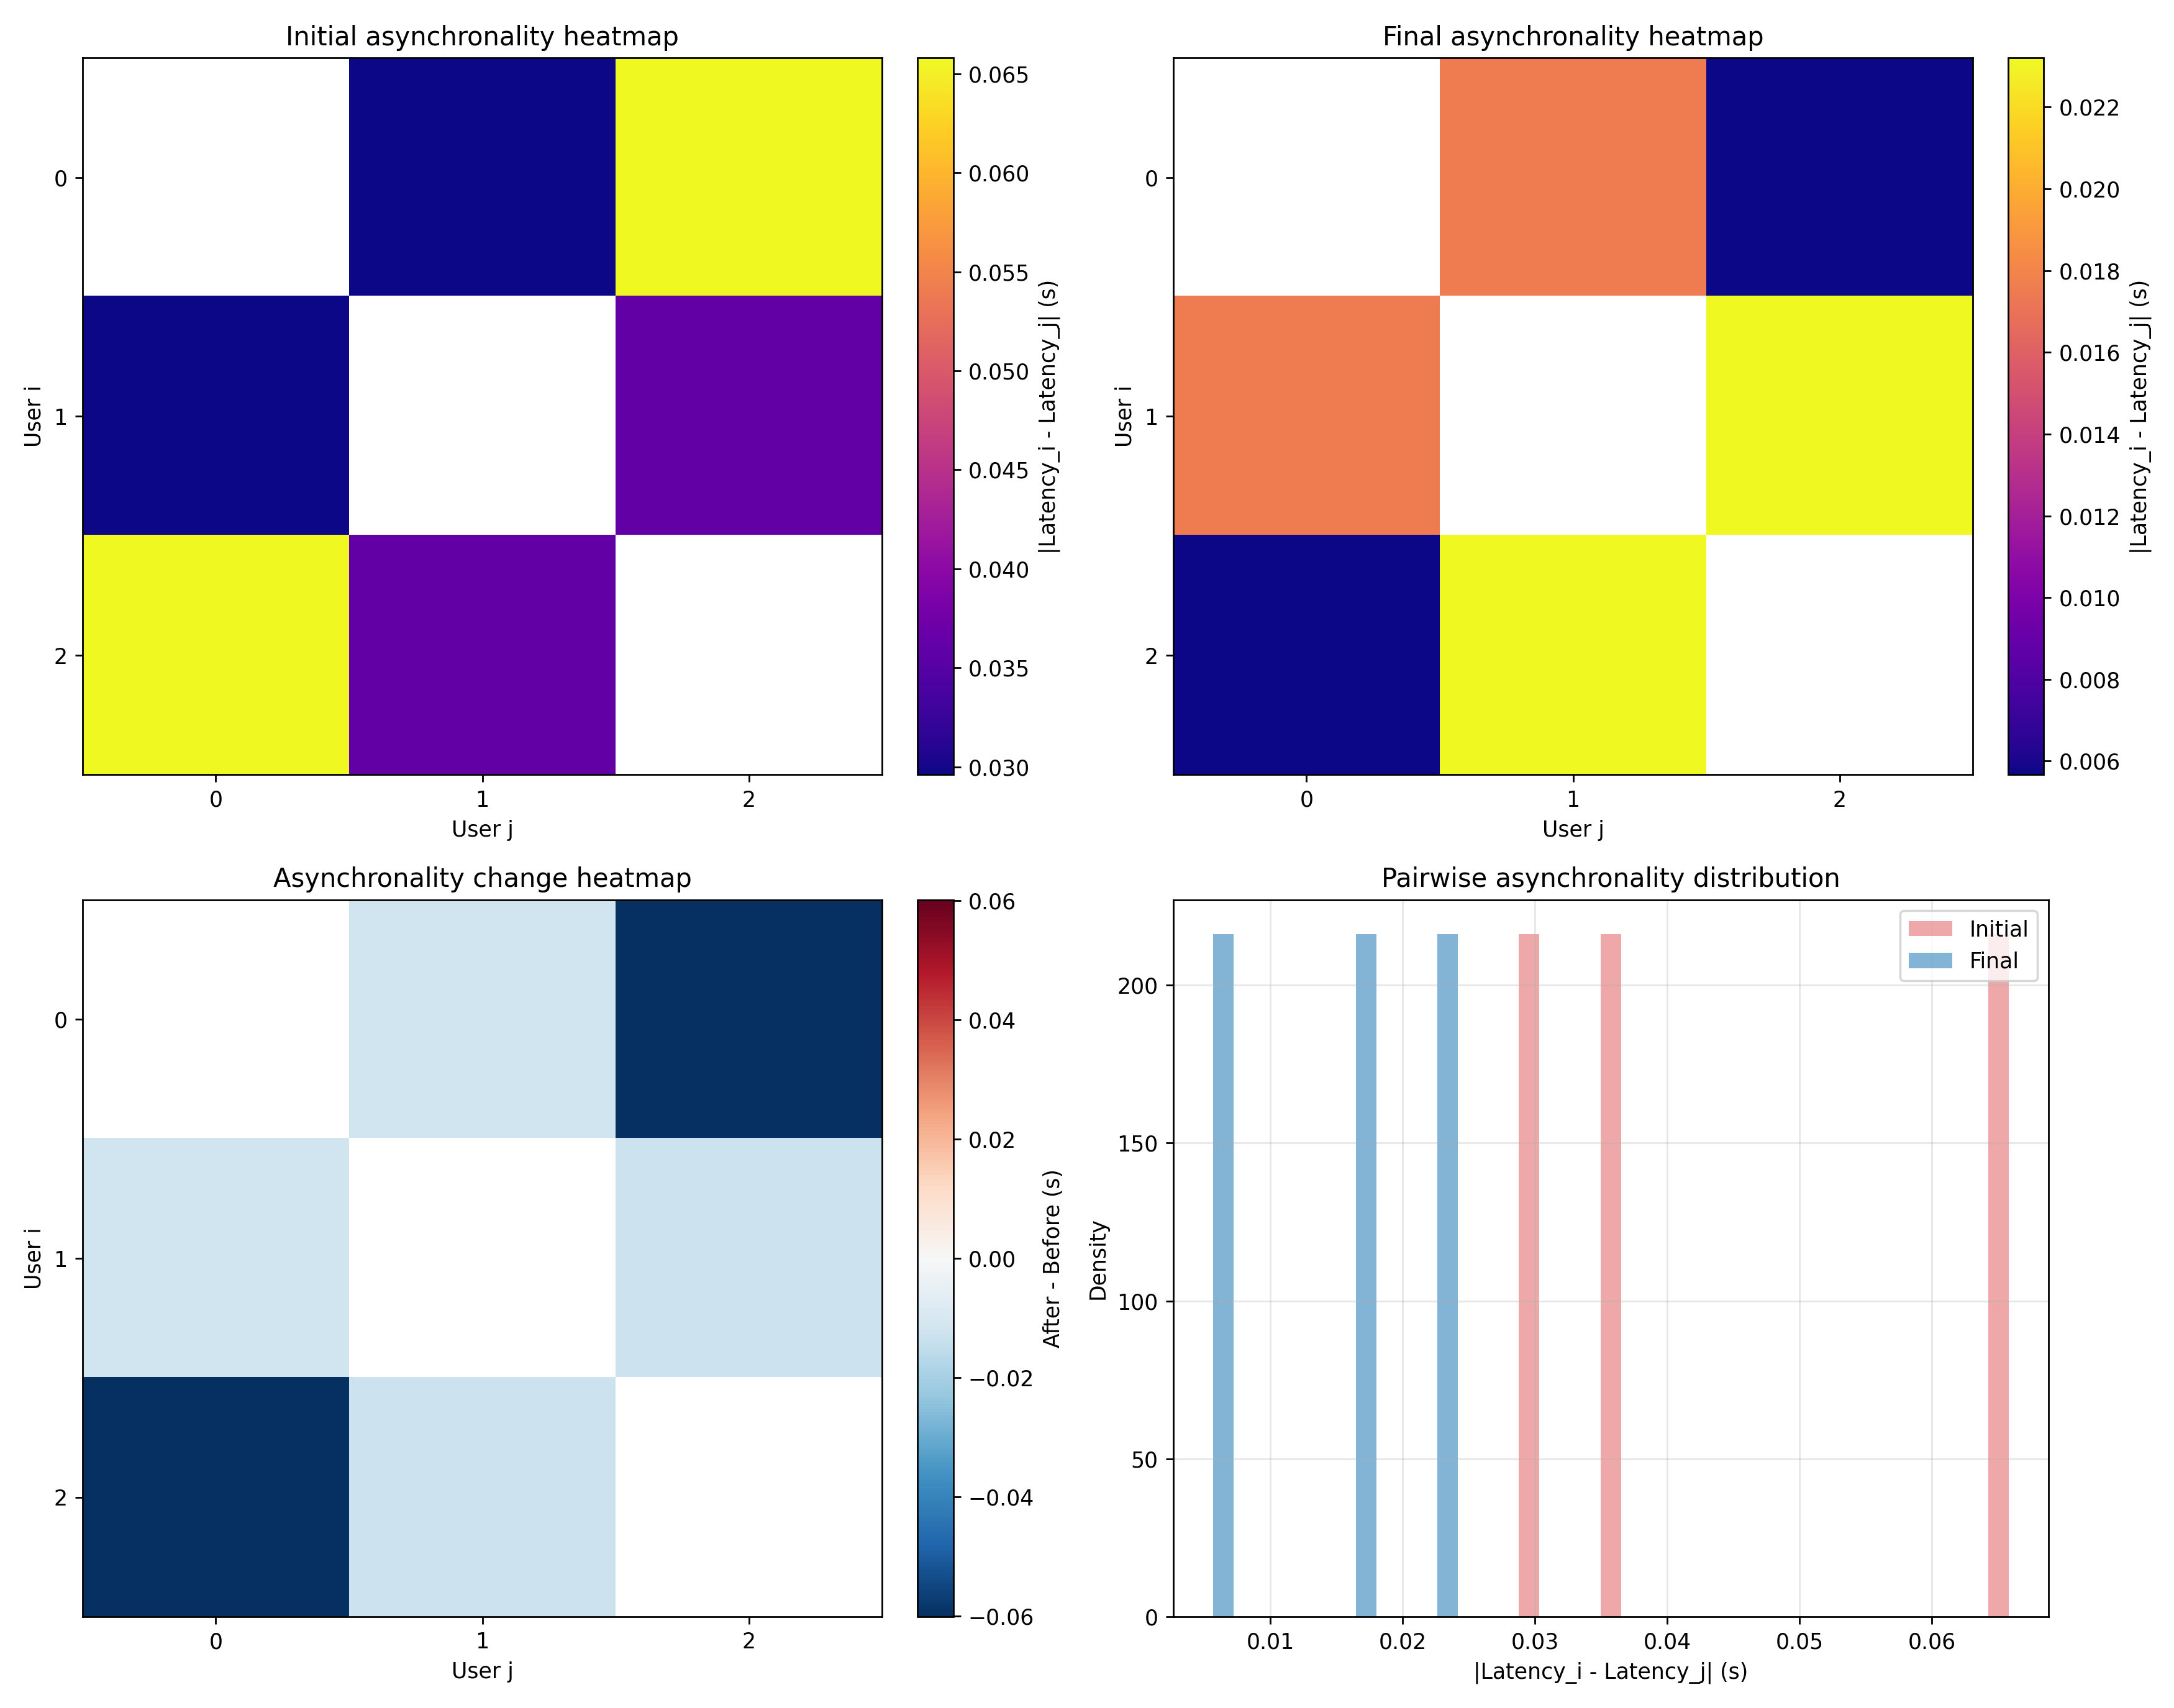
\includegraphics[width=\textwidth]{dl_payload_async_training_testing.png}
    \caption{Training + Testing Method}
\end{subfigure}
\caption{Downlink payload-completion asynchronality comparison. The benchmark produces the tightest final alignment, while the \emph{Training + Testing Method} still leaves a wider residual delay spread.}
\label{fig:dl-payload-asynchronality}
\end{figure}

In downlink continuous communication, the synchronization behavior is weaker.
The benchmark still improves the final asynchronality sum, from \(0.020000\) s
to \(0.016533\) s, but the \emph{Training + Testing Method} moves in the wrong
direction and finishes at \(0.025467\) s. This makes continuous communication
the downlink case where the benchmark advantage is still present but much less
dramatic than in payload completion.

\begin{figure}[H]
\centering
\begin{subfigure}[t]{0.48\textwidth}
    \centering
    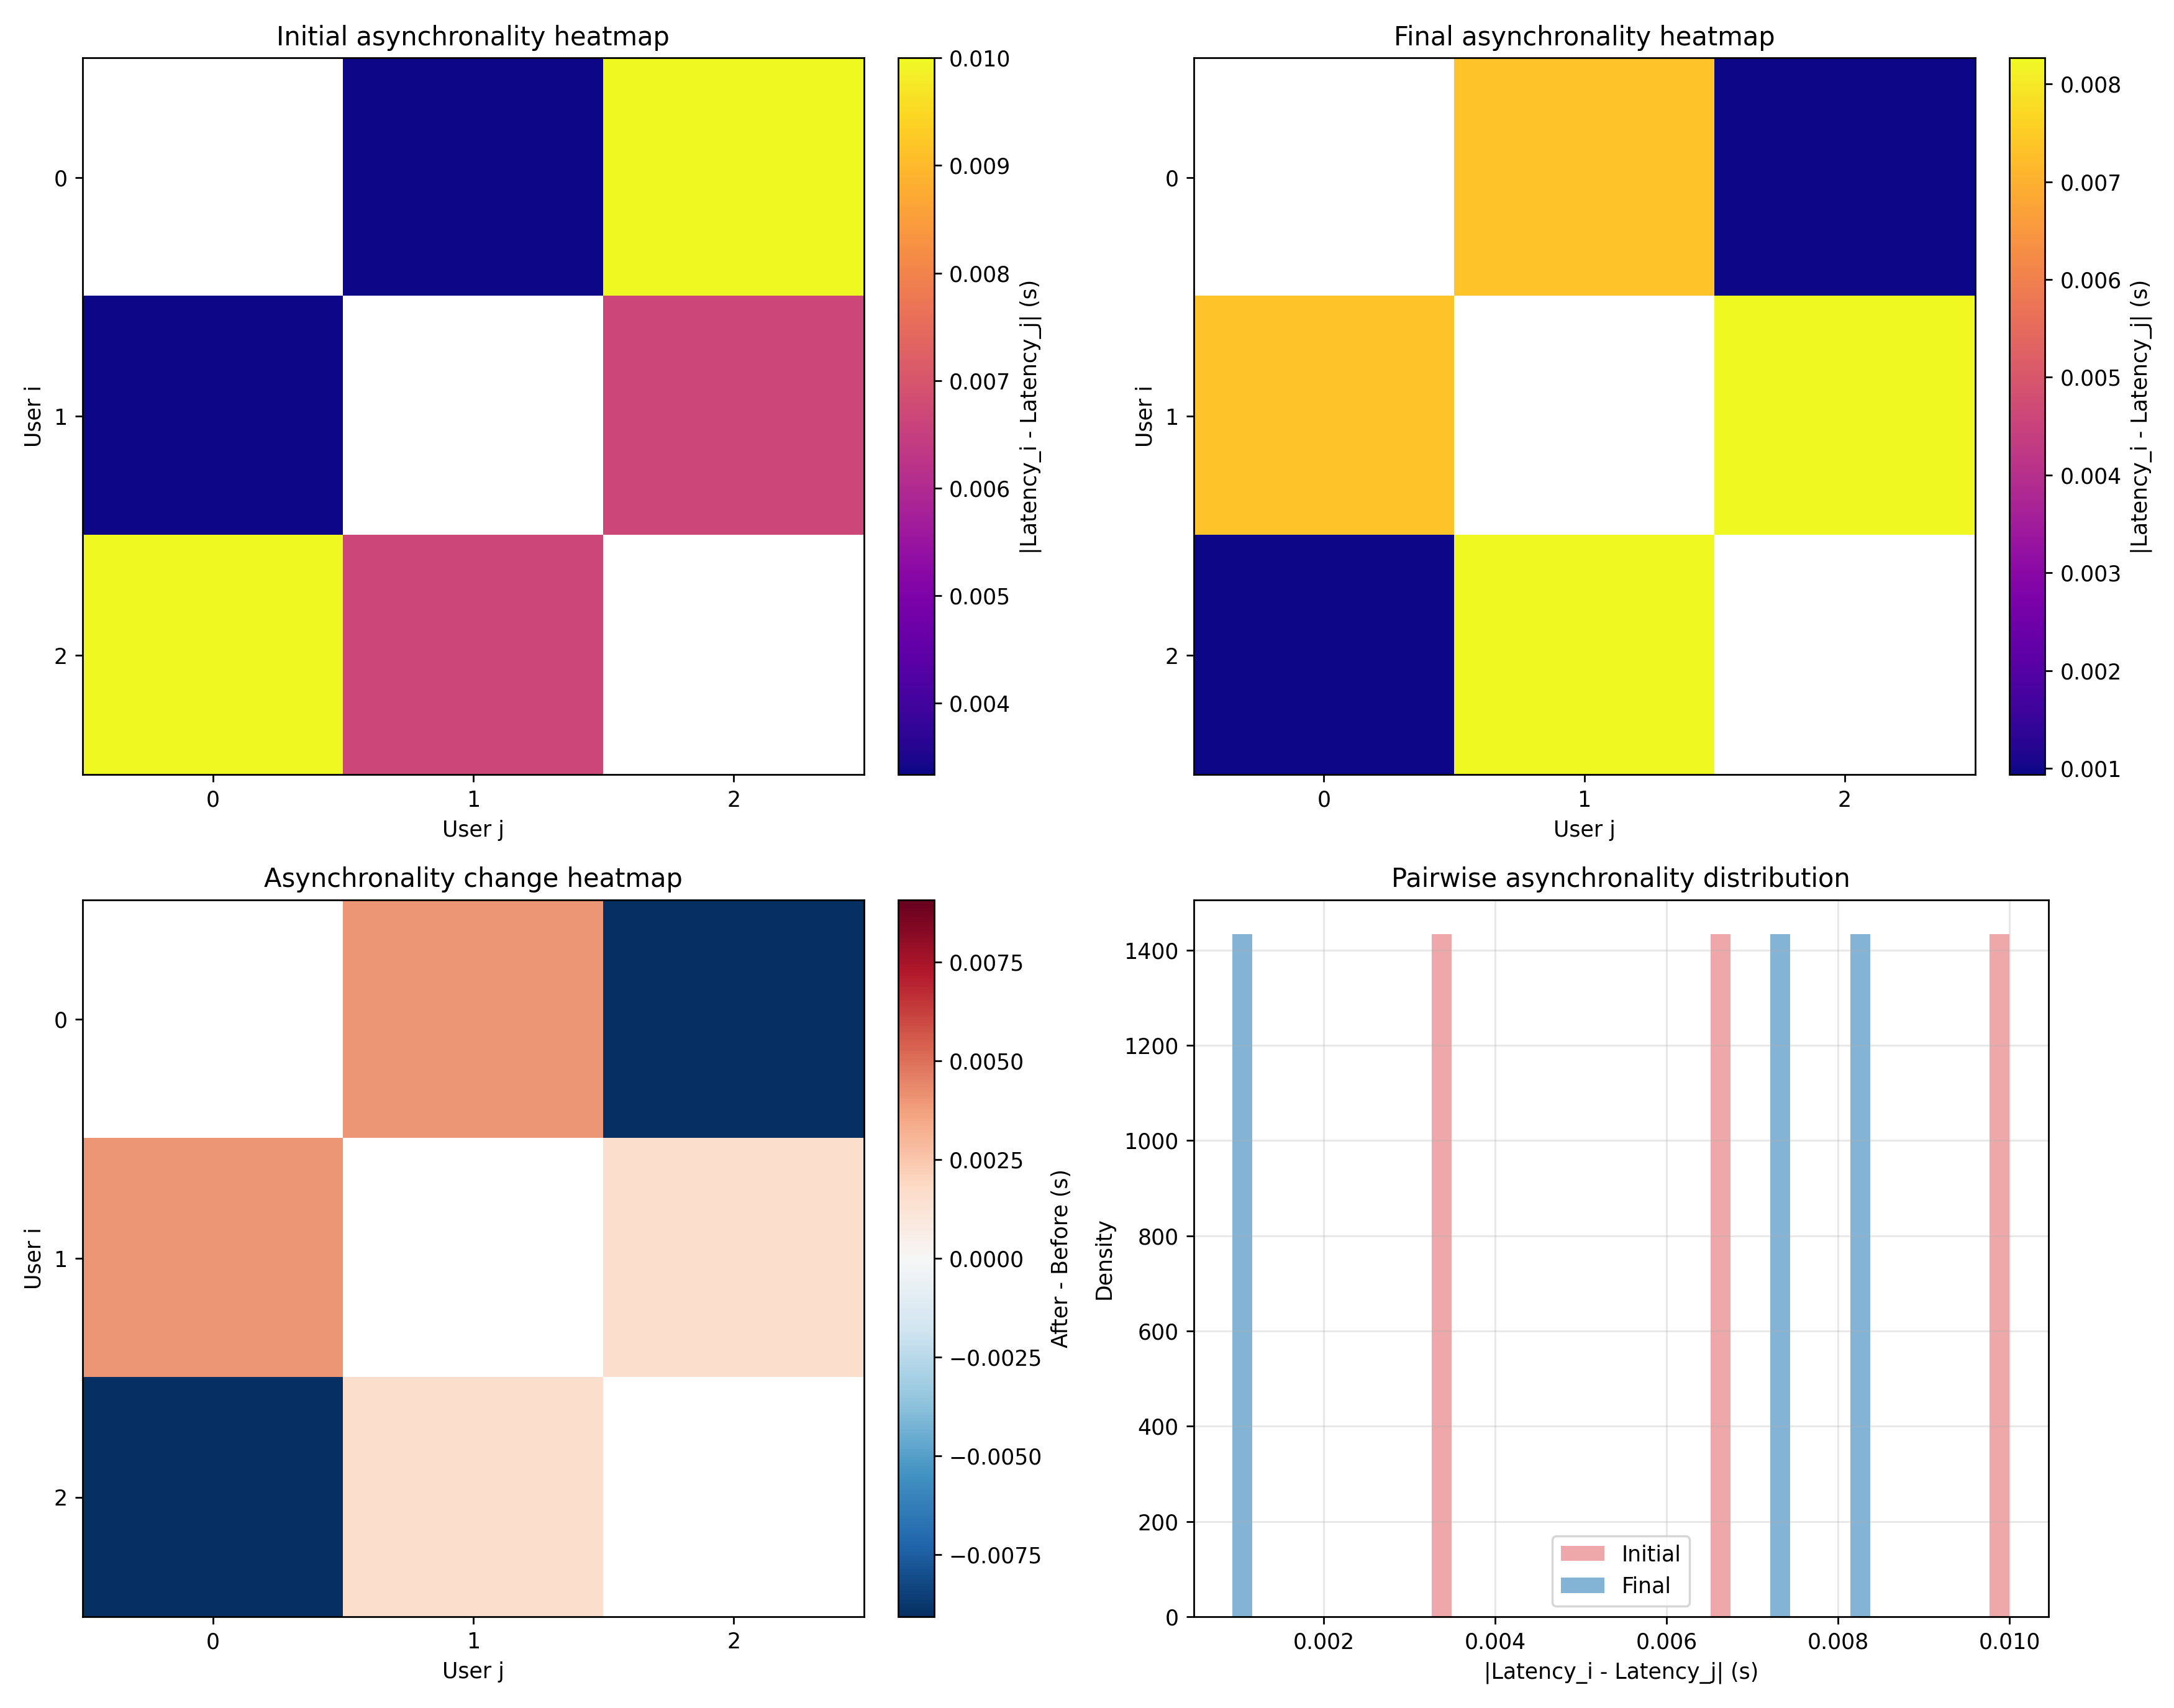
\includegraphics[width=\textwidth]{dl_continuous_async_training_only.png}
    \caption{Training Only Method}
\end{subfigure}
\hfill
\begin{subfigure}[t]{0.48\textwidth}
    \centering
    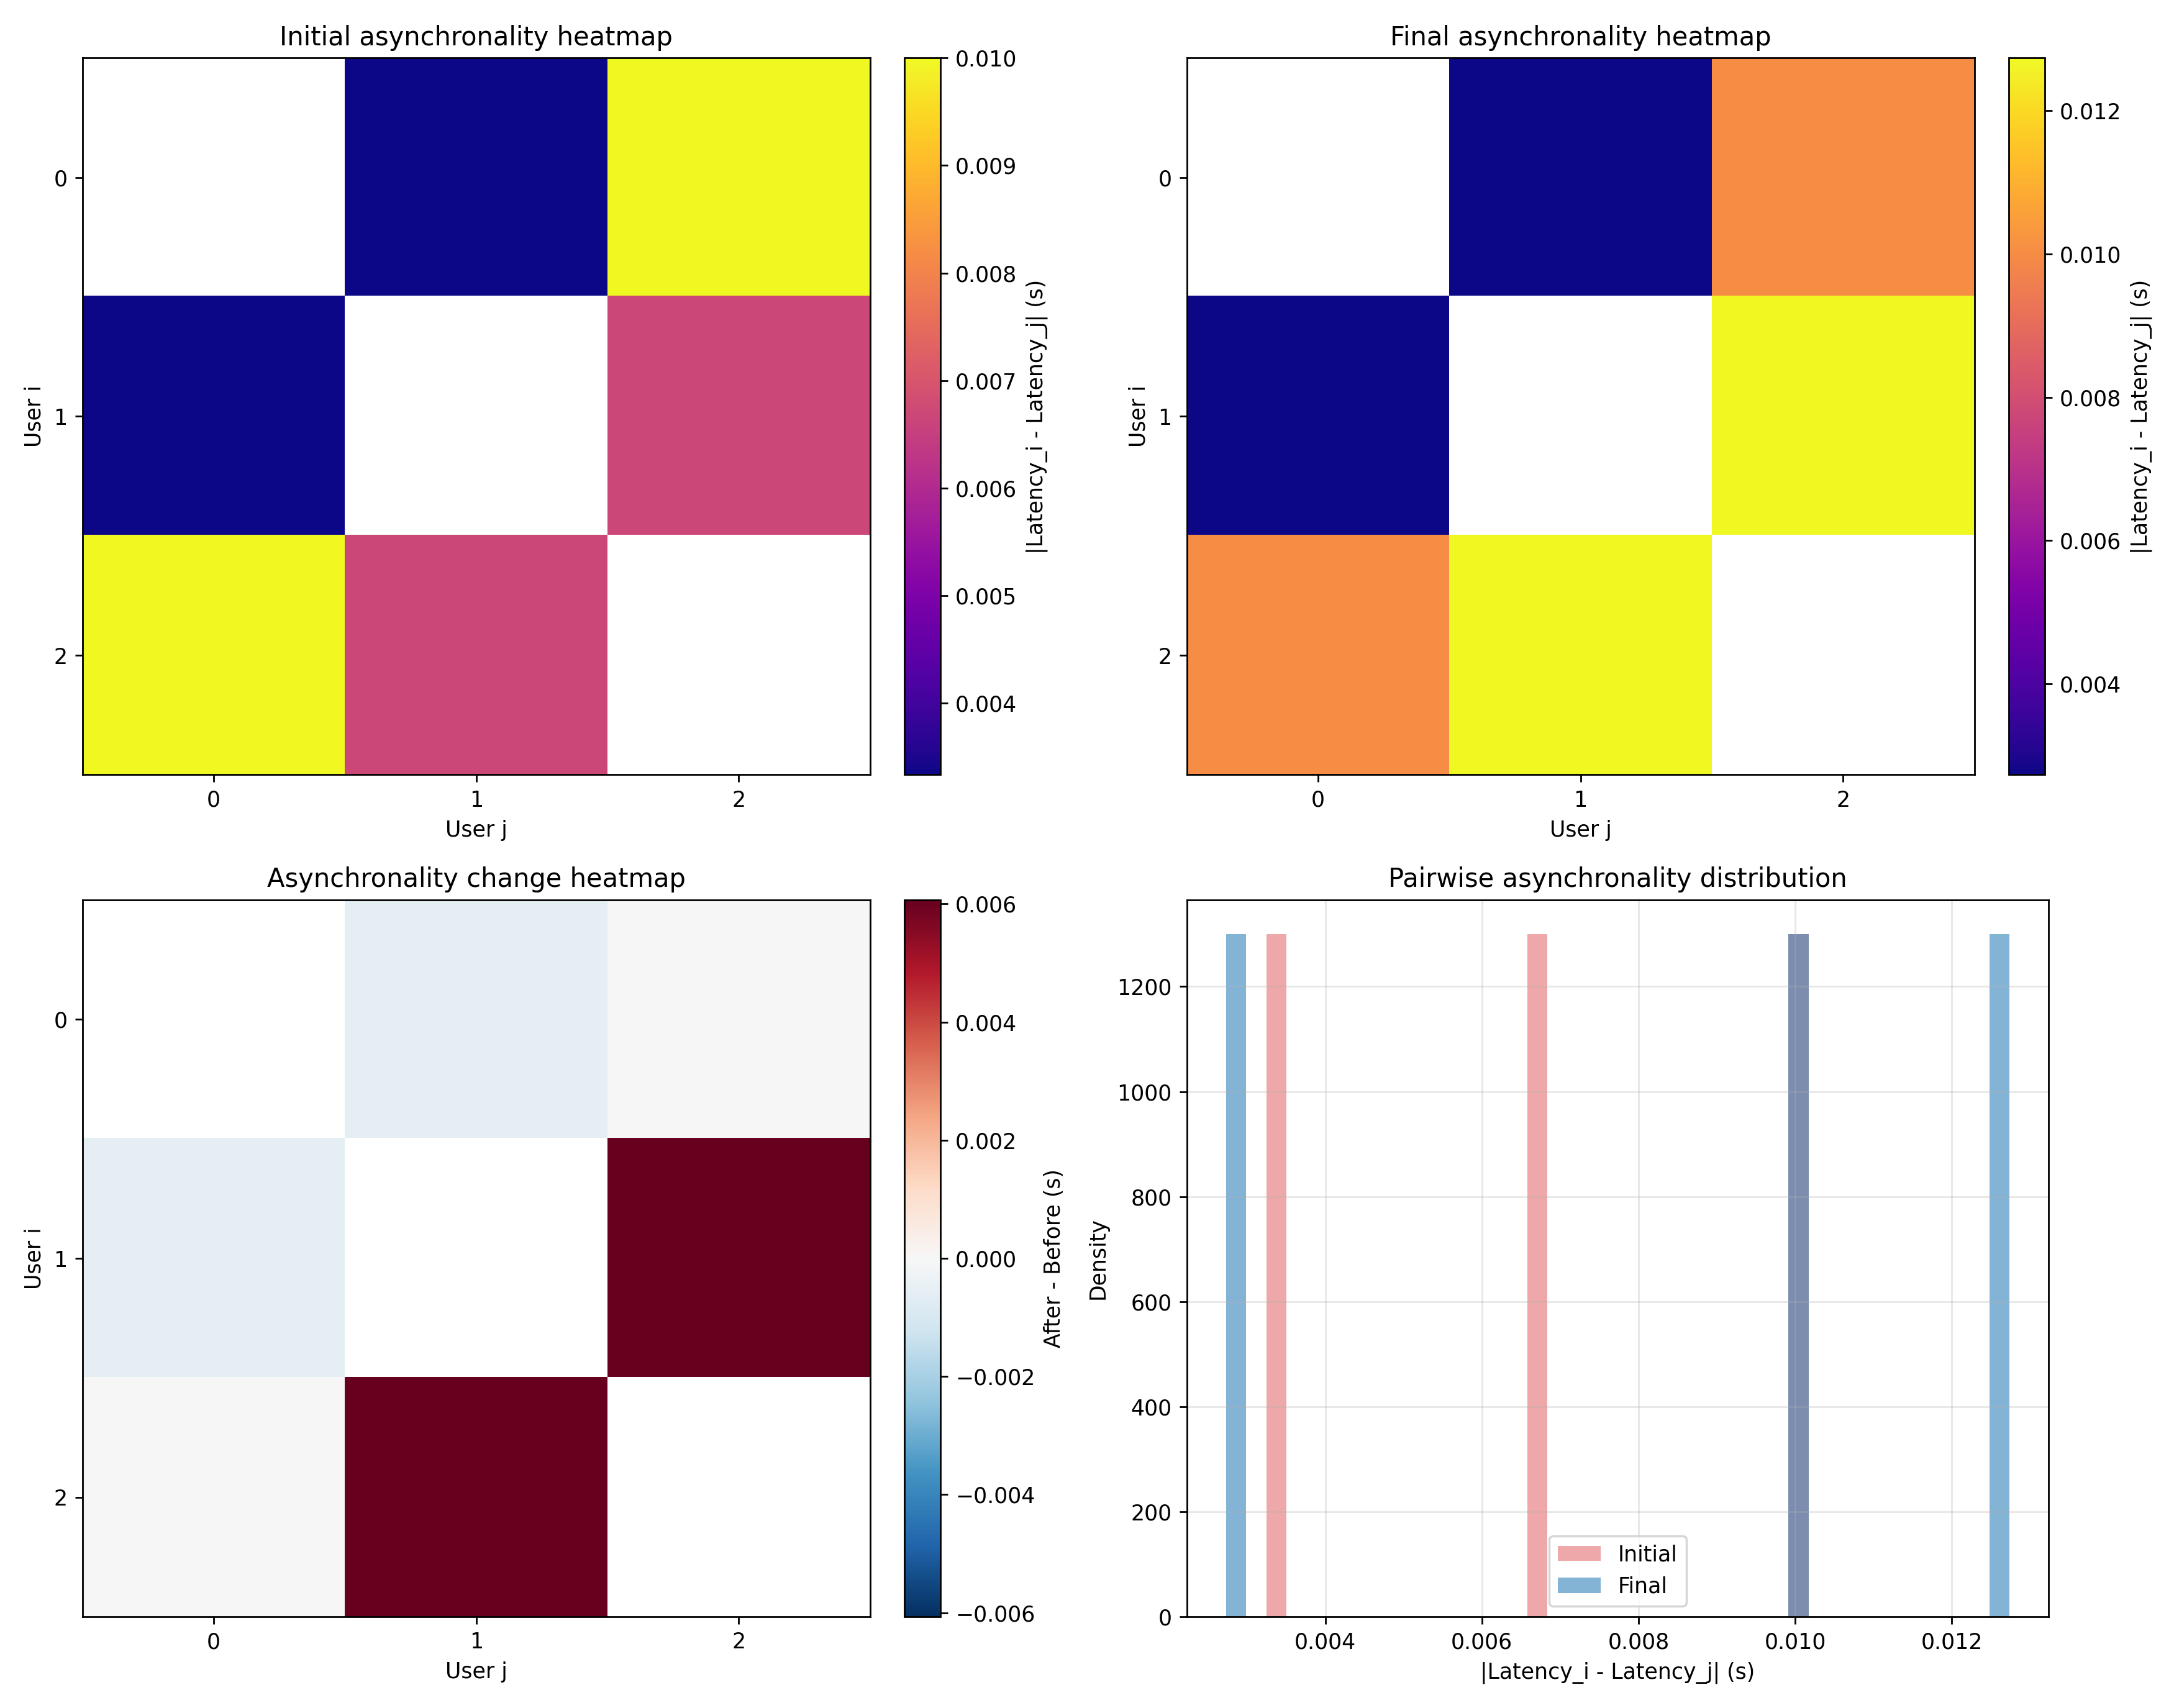
\includegraphics[width=\textwidth]{dl_continuous_async_training_testing.png}
    \caption{Training + Testing Method}
\end{subfigure}
\caption{Downlink continuous-communication asynchronality comparison. The benchmark gives a modest synchronization gain, whereas the \emph{Training + Testing Method} finishes with a larger residual spread than the initial baseline.}
\label{fig:dl-continuous-asynchronality}
\end{figure}

\subsection{Uplink}

The uplink results are much tighter across methods. In payload completion,
both methods start from \(0.016667\) s and finish at \(0.015333\) s, so the
final synchronization outcome is effectively the same. This matches the small
latency gap reported earlier and suggests that, in this case, the testing-stage
method preserves the benchmark synchronization pattern well.

\begin{figure}[H]
\centering
\begin{subfigure}[t]{0.48\textwidth}
    \centering
    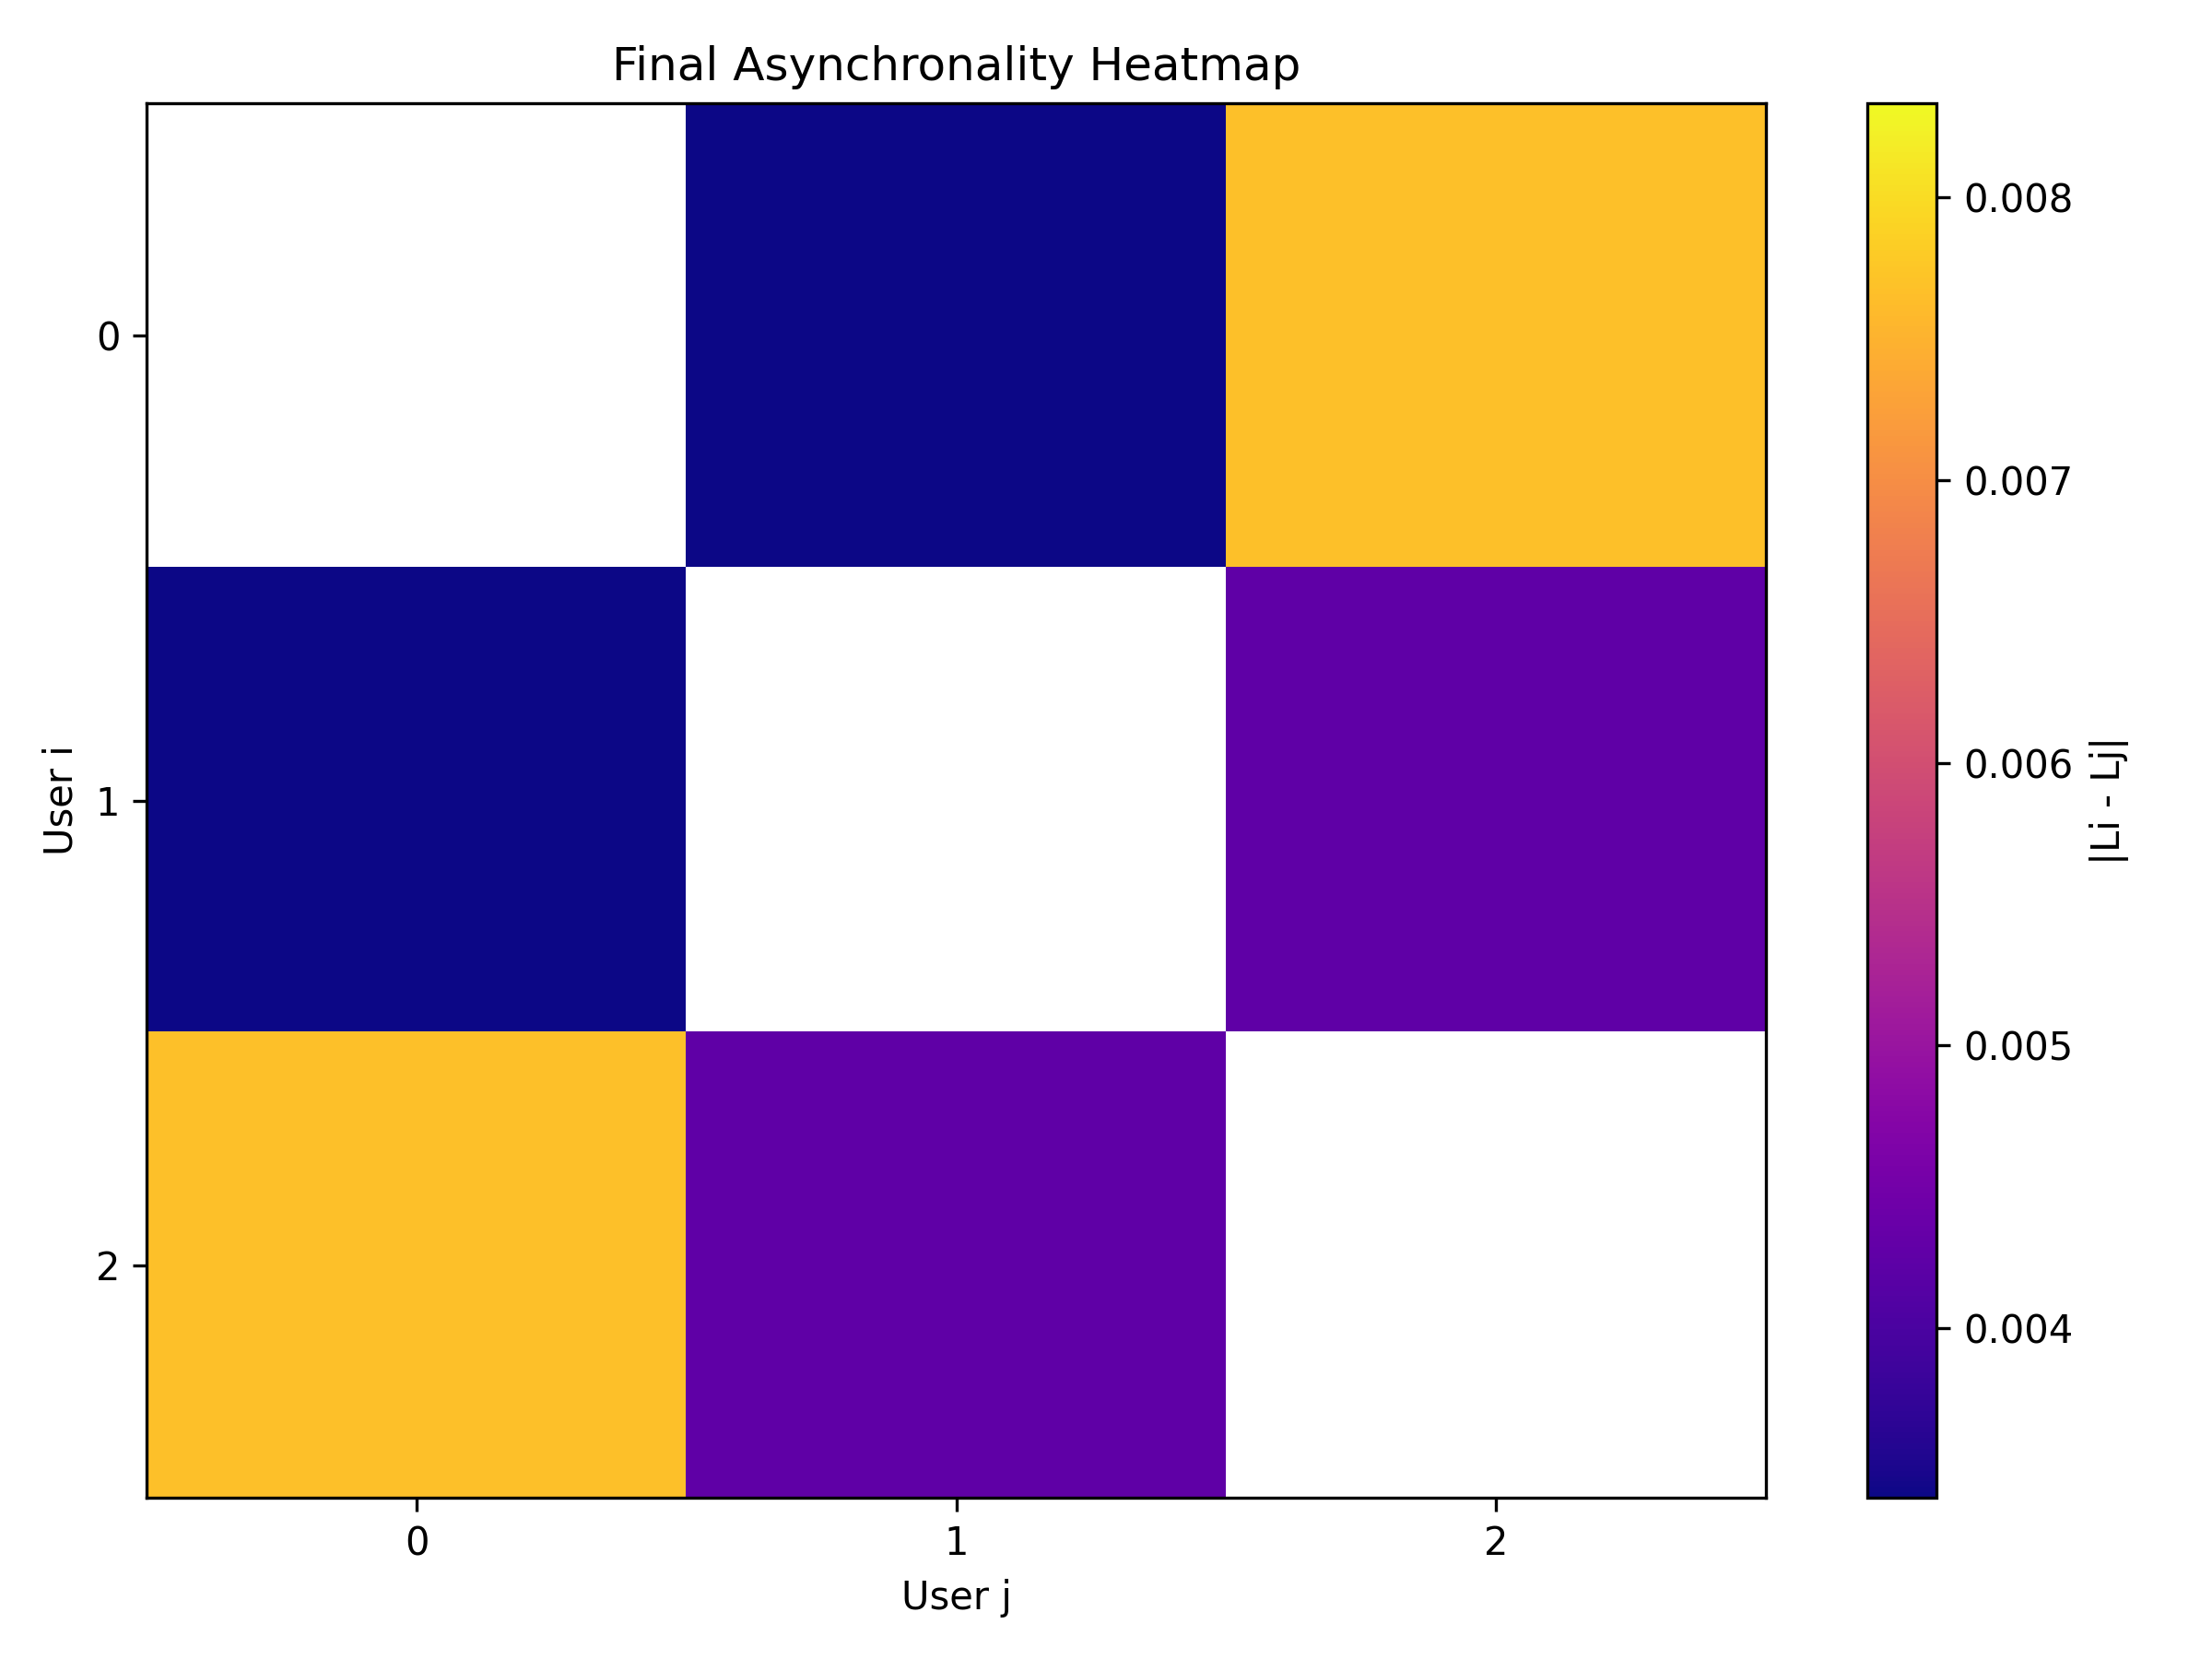
\includegraphics[width=\textwidth]{ul_payload_async_training_only.png}
    \caption{Training Only Method}
\end{subfigure}
\hfill
\begin{subfigure}[t]{0.48\textwidth}
    \centering
    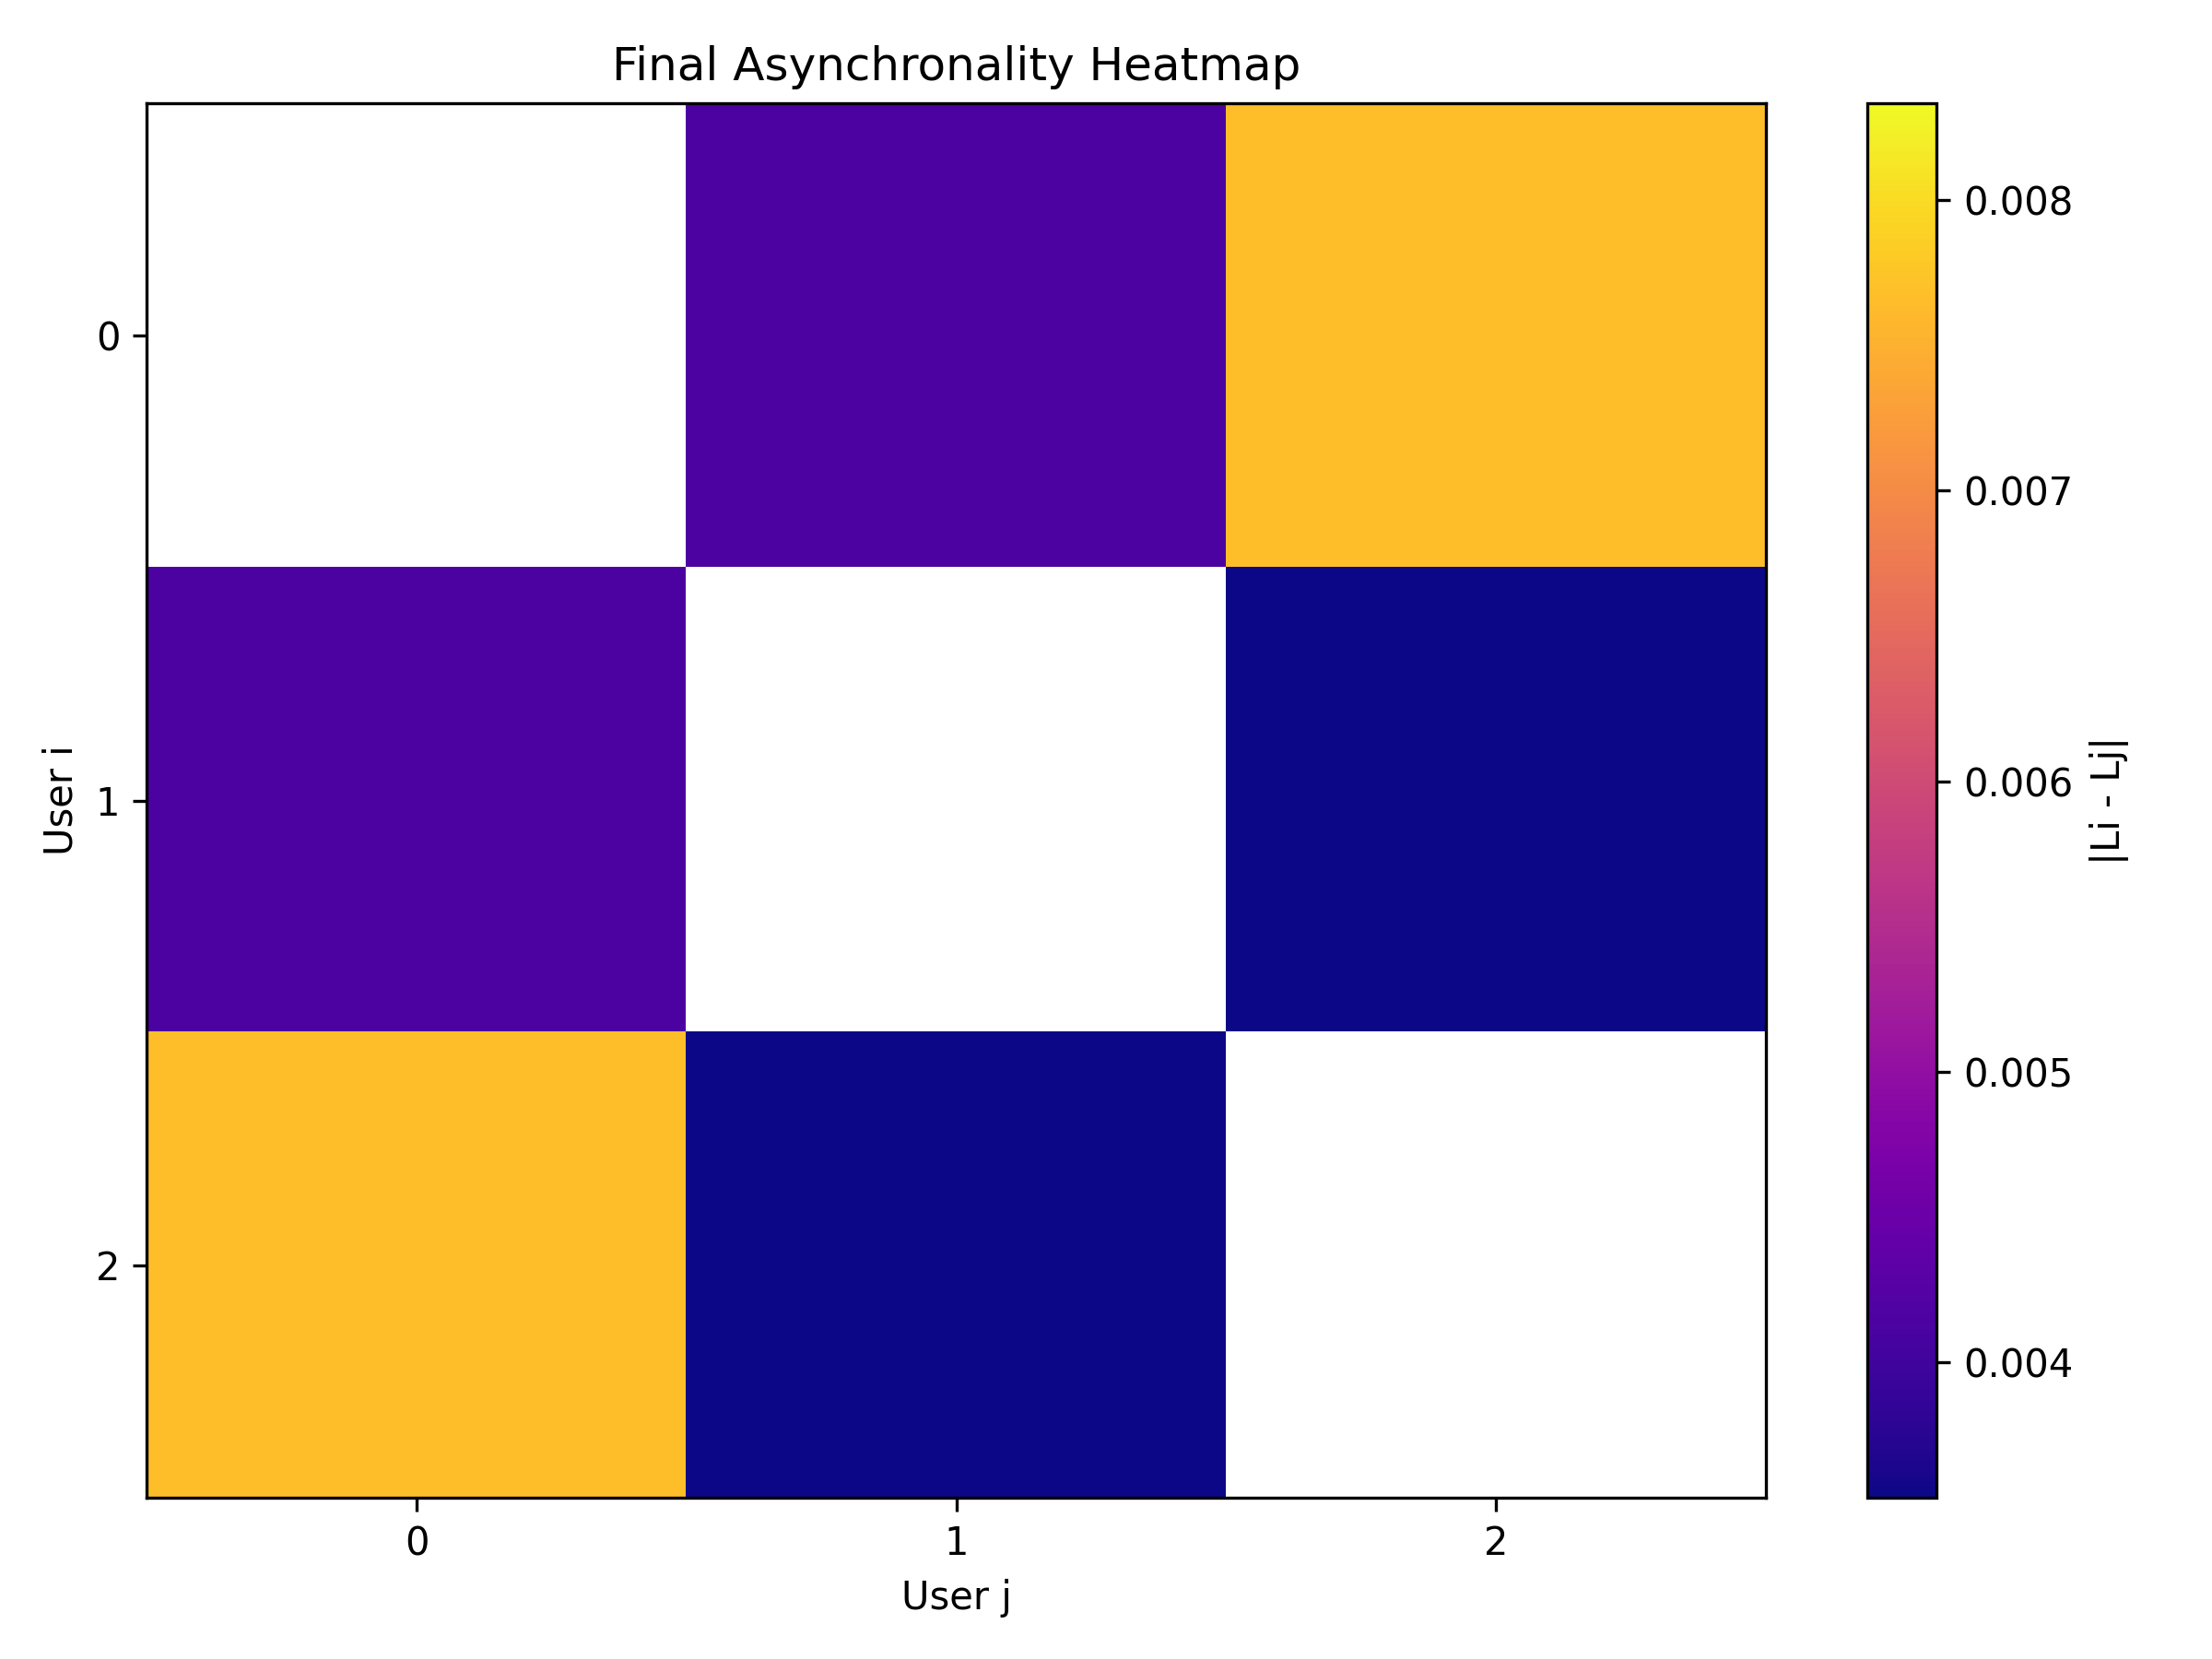
\includegraphics[width=\textwidth]{ul_payload_async_training_testing.png}
    \caption{Training + Testing Method}
\end{subfigure}
\caption{Uplink payload-completion asynchronality comparison. Both methods end with essentially the same final synchronization pattern.}
\label{fig:ul-payload-asynchronality}
\end{figure}

In uplink continuous communication, the benchmark remains strong, but the
\emph{Training + Testing Method} is slightly better on this metric. The final
asynchronality sum is \(0.016267\) s for the benchmark and \(0.015867\) s for
the \emph{Training + Testing Method}. The margin is small, but it shows that
the uplink fixed-horizon case does not follow the same benchmark dominance seen
in the downlink.

\begin{figure}[H]
\centering
\begin{subfigure}[t]{0.48\textwidth}
    \centering
    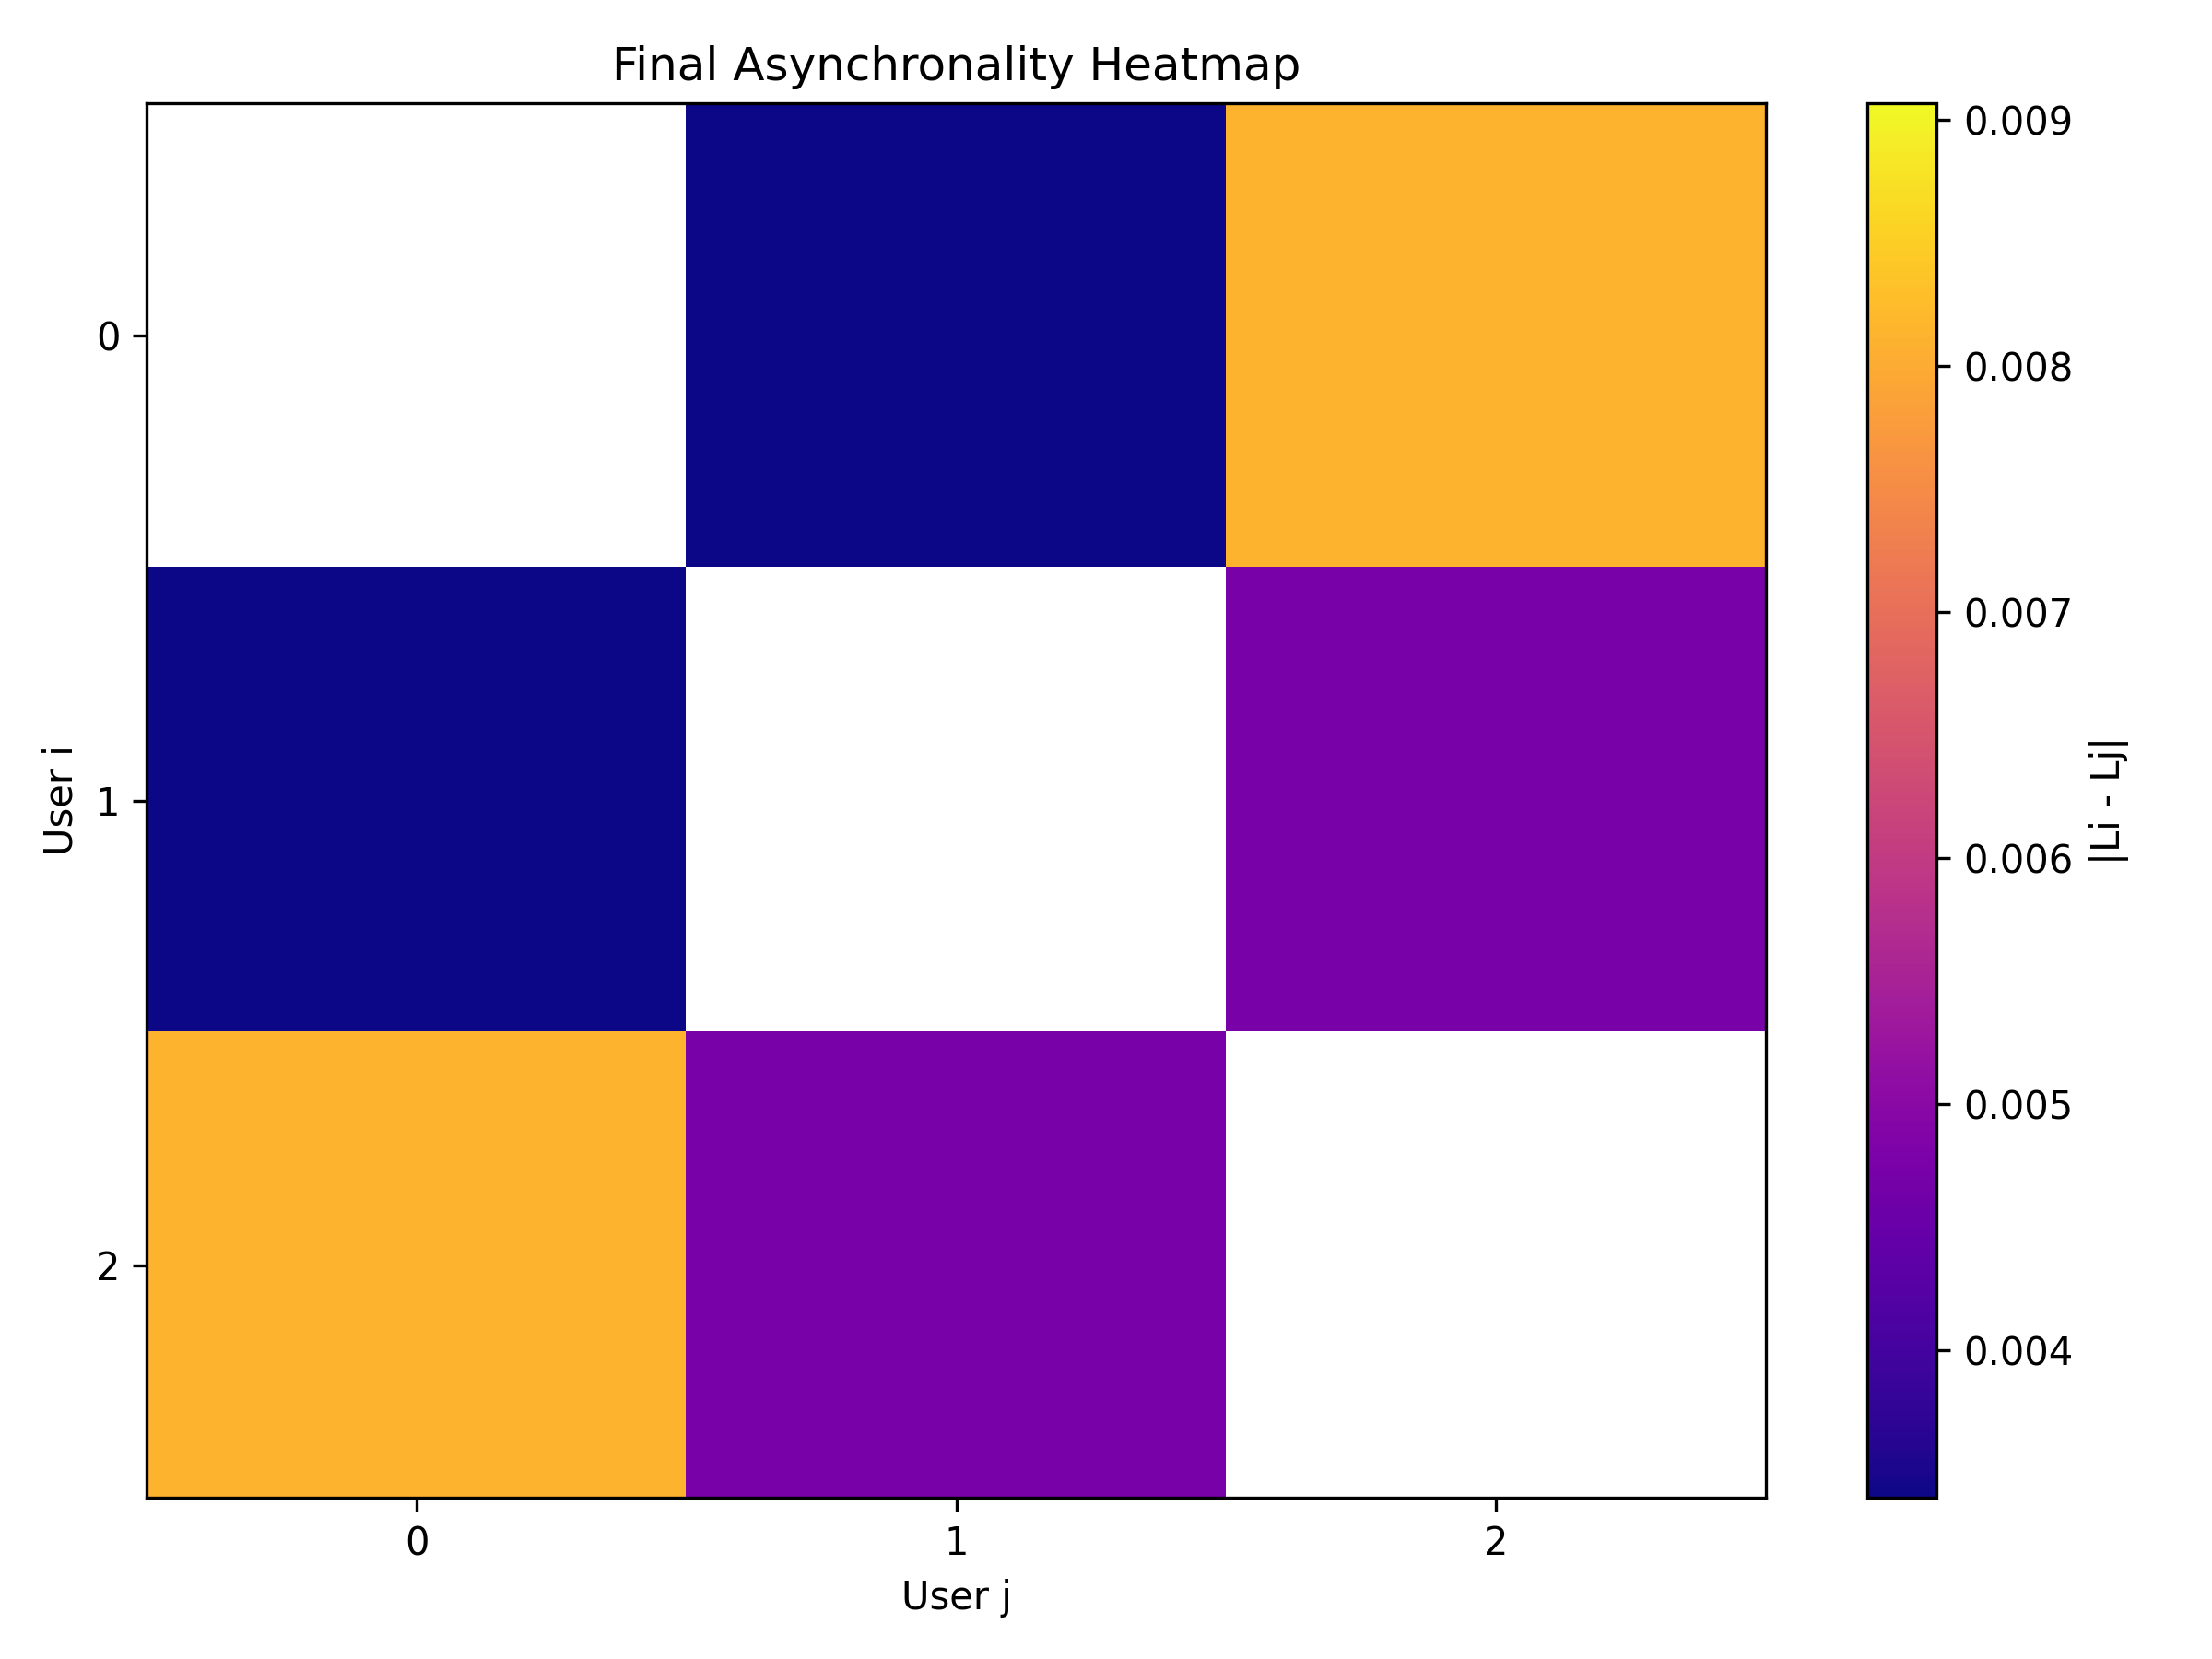
\includegraphics[width=\textwidth]{ul_continuous_async_training_only.png}
    \caption{Training Only Method}
\end{subfigure}
\hfill
\begin{subfigure}[t]{0.48\textwidth}
    \centering
    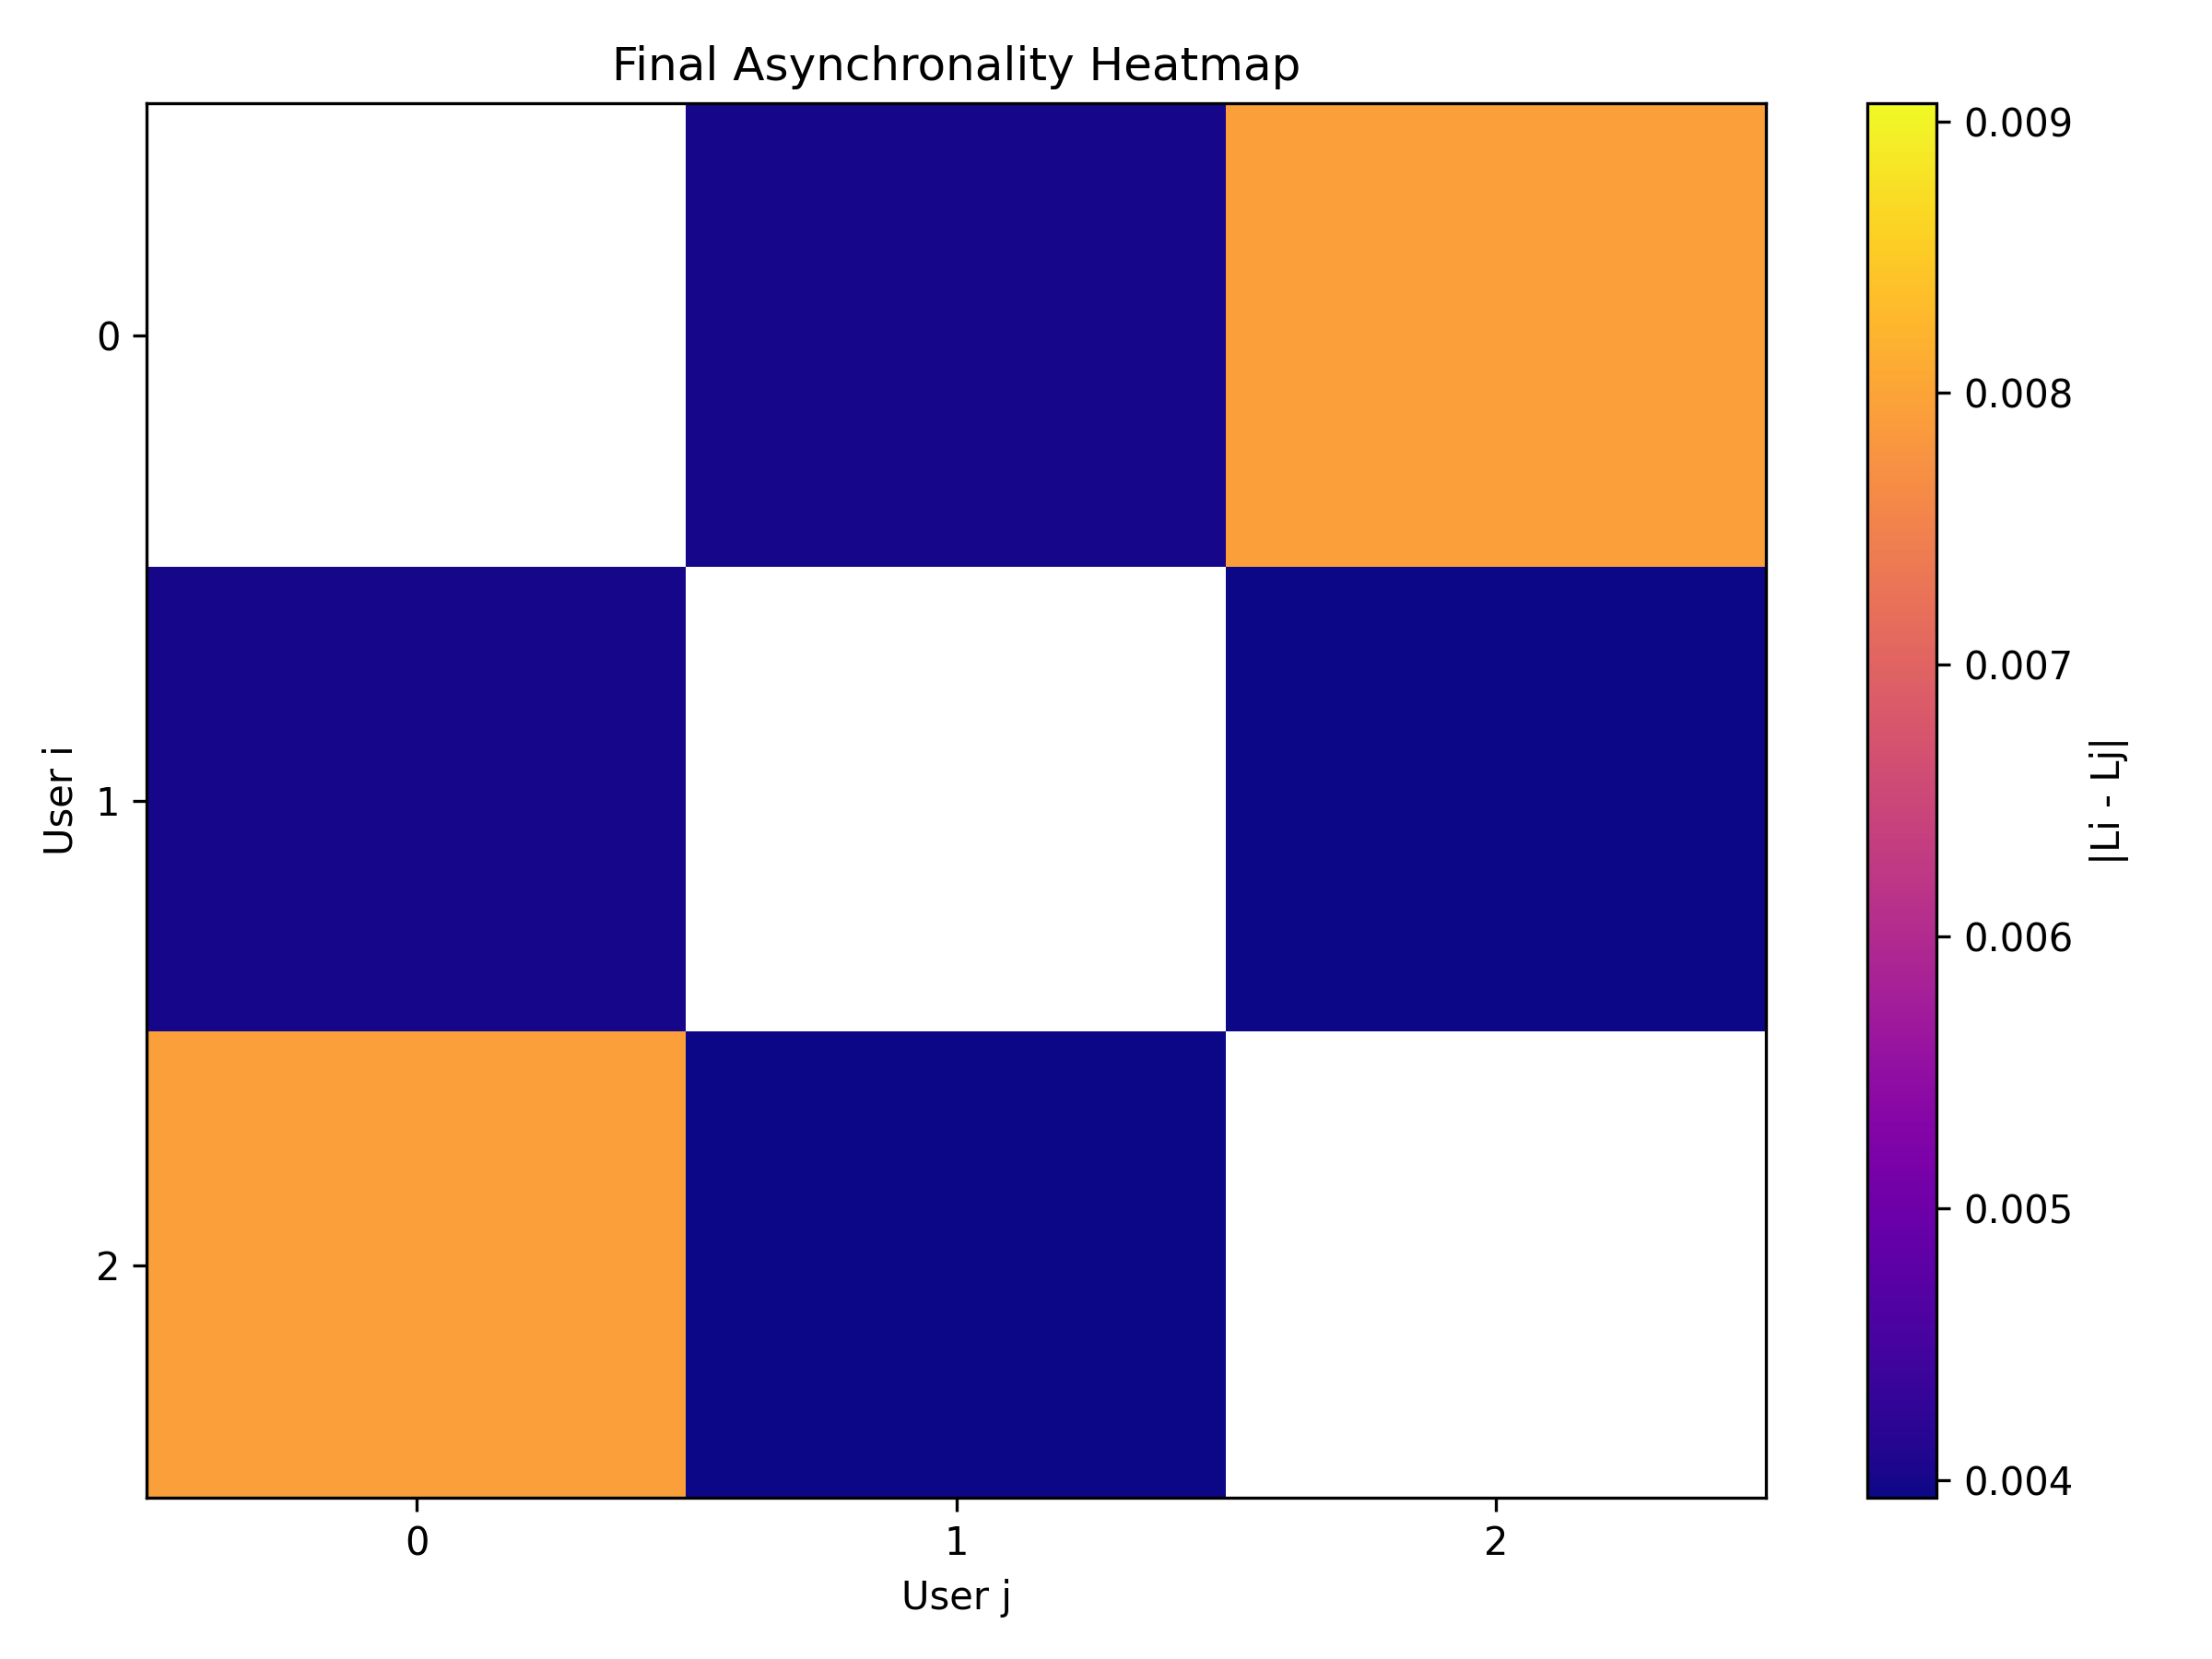
\includegraphics[width=\textwidth]{ul_continuous_async_training_testing.png}
    \caption{Training + Testing Method}
\end{subfigure}
\caption{Uplink continuous-communication asynchronality comparison. The two methods remain close, with a small final advantage for the \emph{Training + Testing Method}.}
\label{fig:ul-continuous-asynchronality}
\end{figure}

\section{Latency Takeaways}

The latency results can be read benchmark-first. In the downlink, the
\emph{Training + Testing Method} still trails the \emph{Training Only Method},
and the gap is most visible in payload completion, where the slower-user
latency tail remains much longer. In continuous communication, the same trend
persists, with the main shortfall again appearing on the higher-latency users.

In the uplink, the picture is much more encouraging. For payload completion,
the \emph{Training + Testing Method} stays close to the benchmark, with only a
small total-latency gap. For continuous communication, it matches the
benchmark exactly at system level. The main takeaway is therefore not a
symmetric head-to-head framing, but a benchmark assessment:
the \emph{Training + Testing Method} is already close in the uplink, while the
downlink remains the main area where further latency improvement is needed.

\end{document}
